\documentclass[12pt,fleqn]{article}
\usepackage{fullpage}
\usepackage{amsmath}
\usepackage{amssymb}
\usepackage{array}

\usepackage{enumitem}
\setlist[enumerate]{leftmargin=*}

\usepackage[most]{tcolorbox}

\newtcbox{\seqbox}{
  on line,
  colback=gray!15,
  colframe=gray!40,
  boxrule=0.3pt,
  arc=3pt,
  left=4pt,right=4pt,top=2pt,bottom=2pt
}

\usepackage{tikz}
\usetikzlibrary{arrows.meta,positioning}
\usepackage{tikz-cd}

\title{How Logic Works: Solutions to Exercises}
\author{Hans Halvorson}

\usepackage[
  colorlinks=true,
  linkcolor=blue!60!black
]{hyperref}

% Starred headings that still go into the TOC
\newcommand{\chaptersection}[1]{%
  \section*{Chapter #1}%
  \addcontentsline{toc}{section}{Chapter #1}%

}
\newcommand{\exercise}[1]{%
  \subsection*{Exercise #1}%
  \addcontentsline{toc}{subsection}{Exercise #1}%
}

\begin{document}
\maketitle

\tableofcontents
\bigskip


\chaptersection{2}

% ---------------------------
% Chapter 2 — Answer Key
% ---------------------------

\exercise{2.1}

\begin{enumerate}
\item \emph{Derive $Q \wedge P$ from $P \wedge Q$.}
\[
\begin{array}{rll}
(1) & P \wedge Q & A \\
(2) & P          & 1\ \wedge E \\
(3) & Q          & 1\ \wedge E \\
(4) & Q \wedge P & 3,2\ \wedge I
\end{array}
\]

\item \emph{Derive $P \wedge (Q \wedge R)$ from $(P \wedge Q)\wedge R$.}
\[
\begin{array}{rll}
(1) & (P \wedge Q)\wedge R & A \\
(2) & P \wedge Q           & 1\ \wedge E \\
(3) & R                    & 1\ \wedge E \\
(4) & P                    & 2\ \wedge E \\
(5) & Q                    & 2\ \wedge E \\
(6) & Q \wedge R           & 5,3\ \wedge I \\
(7) & P \wedge (Q \wedge R)& 4,6\ \wedge I
\end{array}
\]
\end{enumerate}


\exercise{2.2}

\begin{enumerate}
\item $P\wedge Q \;\vdash\; Q\vee R$
\[
\begin{array}{rll}
(1) & P\wedge Q & A \\
(2) & Q         & 1\ \wedge E \\
(3) & Q\vee R   & 2\ \vee I
\end{array}
\]

\item $P\wedge Q \;\vdash\; (P\vee R)\wedge(Q\vee R)$
\[
\begin{array}{rll}
(1) & P\wedge Q                 & A \\
(2) & P                         & 1\ \wedge E \\
(3) & Q                         & 1\ \wedge E \\
(4) & P\vee R                   & 2\ \vee I \\
(5) & Q\vee R                   & 3\ \vee I \\
(6) & (P\vee R)\wedge(Q\vee R)  & 4,5\ \wedge I
\end{array}
\]

\item $P \;\vdash\; Q\vee(P\vee Q)$
\[
\begin{array}{rll}
(1) & P           & A \\
(2) & P\vee Q     & 1\ \vee I \\
(3) & Q\vee(P\vee Q) & 2\ \vee I
\end{array}
\]

\item $P \;\vdash\; (P\vee R)\wedge(P\vee Q)$
\[
\begin{array}{rll}
(1) & P                 & A \\
(2) & P\vee R           & 1\ \vee I \\
(3) & P\vee Q           & 1\ \vee I \\
(4) & (P\vee R)\wedge(P\vee Q) & 2,3\ \wedge I
\end{array}
\]
\end{enumerate}


\exercise{2.3}

\begin{enumerate}
\item $P\to(Q\to R),\; P\to Q,\; P \;\vdash\; R$
\[
\begin{array}{rll}
(1) & P\to(Q\to R) & A \\
(2) & P\to Q       & A \\
(3) & P            & A \\
(4) & Q\to R       & 1,3\ MP \\
(5) & Q            & 2,3\ MP \\
(6) & R            & 4,5\ MP
\end{array}
\]

\item $(A\vee B)\to T,\; Z\to A,\; T\to W,\; Z \;\vdash\; W$
\[
\begin{array}{rll}
(1) & (A\vee B)\to T & A \\
(2) & Z\to A         & A \\
(3) & T\to W         & A \\
(4) & Z              & A \\
(5) & A              & 2,4\ MP \\
(6) & A\vee B         & 5\ \vee I \\
(7) & T              & 1,6\ MP \\
(8) & W              & 3,7\ MP
\end{array}
\]

\item $(A\to B)\wedge(C\to A),\; (C\wedge(W\to Z))\wedge W \;\vdash\; (B\vee D)\wedge(Z\vee E)$
\[
\begin{array}{rll}
(1)  & (A\to B)\wedge(C\to A)            & A \\
(2)  & (C\wedge(W\to Z))\wedge W          & A \\
(3)  & A\to B                             & 1\ \wedge E \\
(4)  & C\to A                             & 1\ \wedge E \\
(5)  & C\wedge(W\to Z)                    & 2\ \wedge E \\
(6)  & W                                  & 2\ \wedge E \\
(7)  & C                                  & 5\ \wedge E \\
(8)  & W\to Z                             & 5\ \wedge E \\
(9)  & A                                  & 4,7\ MP \\
(10) & B                                  & 3,9\ MP \\
(11) & B\vee D                            & 10\ \vee I \\
(12) & Z                                  & 8,6\ MP \\
(13) & Z\vee E                            & 12\ \vee I \\
(14) & (B\vee D)\wedge(Z\vee E)           & 11,13\ \wedge I
\end{array}
\]

\item $P\to(P\to Q),\; P \;\vdash\; Q$
\[
\begin{array}{rll}
(1) & P\to(P\to Q) & A \\
(2) & P            & A \\
(3) & P\to Q       & 1,2\ MP \\
(4) & Q            & 3,2\ MP
\end{array}
\]

\item $P\wedge(P\to Q) \;\vdash\; P\wedge Q$
\[
\begin{array}{rll}
(1) & P\wedge(P\to Q) & A \\
(2) & P               & 1\ \wedge E \\
(3) & P\to Q          & 1\ \wedge E \\
(4) & Q               & 3,2\ MP \\
(5) & P\wedge Q       & 2,4\ \wedge I
\end{array}
\]
\end{enumerate}


\exercise{2.4}

\emph{Prove $Q\to(P\to R),\; \neg R\wedge Q \;\vdash\; \neg P$.}
\[
\begin{array}{rll}
(1) & Q\to(P\to R) & A \\
(2) & \neg R\wedge Q & A \\
(3) & Q            & 2\ \wedge E \\
(4) & \neg R       & 2\ \wedge E \\
(5) & P\to R       & 1,3\ MP \\
(6) & \neg P       & 5,4\ MT
\end{array}
\]


\exercise{2.5}

\begin{enumerate}
\item $P\wedge(Q\wedge R) \dashv\vdash (P\wedge Q)\wedge R$

\smallskip
($\Rightarrow$)
\[
\begin{array}{rll}
(1) & P\wedge(Q\wedge R) & A \\
(2) & P                  & 1\ \wedge E \\
(3) & Q\wedge R           & 1\ \wedge E \\
(4) & Q                  & 3\ \wedge E \\
(5) & R                  & 3\ \wedge E \\
(6) & P\wedge Q          & 2,4\ \wedge I \\
(7) & (P\wedge Q)\wedge R& 6,5\ \wedge I
\end{array}
\]

\smallskip
($\Leftarrow$)
\[
\begin{array}{rll}
(1) & (P\wedge Q)\wedge R & A \\
(2) & P\wedge Q           & 1\ \wedge E \\
(3) & R                   & 1\ \wedge E \\
(4) & P                   & 2\ \wedge E \\
(5) & Q                   & 2\ \wedge E \\
(6) & Q\wedge R            & 5,3\ \wedge I \\
(7) & P\wedge(Q\wedge R)   & 4,6\ \wedge I
\end{array}
\]

\item $P \dashv\vdash P\wedge P$

\smallskip
($\Rightarrow$)
\[
\begin{array}{rll}
(1) & P      & A \\
(2) & P\wedge P & 1,1\ \wedge I
\end{array}
\]

\smallskip
($\Leftarrow$)
\[
\begin{array}{rll}
(1) & P\wedge P & A \\
(2) & P         & 1\ \wedge E
\end{array}
\]
\end{enumerate}


\exercise{2.6}

\begin{enumerate}
\item $\neg(\neg R \to H)$
\item $\neg E \to S$ \quad (equivalently: $E\vee S$)
\item $\neg P \wedge \neg S$
\item $A \to (H\vee B)$
\item $K \wedge \bigl((M\wedge F)\vee \neg F\bigr)$
\item $\neg(H\wedge D)$
\end{enumerate}


\exercise{2.7}

\begin{enumerate}
\item $\neg\neg Q\to P,\; \neg P \;\vdash\; \neg Q$
\[
\begin{array}{rll}
(1) & \neg\neg Q\to P & A \\
(2) & \neg P          & A \\
(3) & \neg\neg\neg Q  & 1,2\ MT \\
(4) & \neg Q          & 3\ DN
\end{array}
\]

\item $P\to(P\to Q),\; P \;\vdash\; Q$
\[
\begin{array}{rll}
(1) & P\to(P\to Q) & A \\
(2) & P            & A \\
(3) & P\to Q       & 1,2\ MP \\
(4) & Q            & 3,2\ MP
\end{array}
\]

\item $(P\wedge P)\to Q,\; P \;\vdash\; Q$
\[
\begin{array}{rll}
(1) & (P\wedge P)\to Q & A \\
(2) & P                & A \\
(3) & P\wedge P         & 2,2\ \wedge I \\
(4) & Q                & 1,3\ MP
\end{array}
\]

\item $P \;\vdash\; Q\vee(\neg\neg P \vee R)$
\[
\begin{array}{rll}
(1) & P                 & A \\
(2) & \neg\neg P         & 1\ DN \\
(3) & \neg\neg P \vee R  & 2\ \vee I \\
(4) & Q \vee (\neg\neg P \vee R) & 3\ \vee I
\end{array}
\]
\end{enumerate}


\exercise{2.8}

\begin{enumerate}
\item $P\to \neg Q,\; \neg P \;\not\vdash\; Q$

Counterexample (English instance):
Let $P$ be “It is raining.” Let $Q$ be “$2+2=5$.”
Then $Q$ is false, so $\neg Q$ is true; hence $P\to\neg Q$ is true.
Also $\neg P$ can be true (suppose it isn’t raining). But $Q$ is false.

\item $P\to R \;\not\vdash\; (P\vee Q)\to R$

Counterexample (English instance):
Let $P$ be “I am on Mars.” (false)
Let $Q$ be “I am on Earth.” (true)
Let $R$ be “$2+2=5$.” (false)
Then $P\to R$ is true (false antecedent), but $(P\vee Q)\to R$ is false
(true antecedent, false consequent).
\end{enumerate}

\chaptersection{3}

\exercise{3.1}

\begin{enumerate}

\item \seqbox{$P\:\vdash \:Q \to (P \wedge Q)$}

  \noindent \begin{tabular}{@{}
      >{\raggedleft\arraybackslash}r
      >{\centering\arraybackslash}p{1.0cm} p{5cm}
      >{\raggedright\arraybackslash}p{3.5cm}}
              1   & (1) & $P$              & A \\
              2   & (2) & $Q$              & A \\
              1,2 & (3) & $P \wedge Q$     & 1,2 $\wedge$I \\
              1   & (4) & $Q \to (P \wedge Q)$ & 2,3 CP \\
\end{tabular}

\item \seqbox{$(P \to Q) \wedge (P \to R) \:\vdash P \:\to (Q \wedge R)$}

  \noindent \begin{tabular}{>{\raggedleft\arraybackslash}r
      >{\centering\arraybackslash}p{1.0cm} p{5cm}
      >{\raggedright\arraybackslash}p{3.5cm}}
1   & (1) & $(P \to Q) \wedge (P \to R)$ & A \\
2   & (2) & $P$              & A \\
1   & (3) & $P \to Q$        & 1 $\wedge$E \\
1   & (4) & $P \to R$        & 1 $\wedge$E \\
1,2 & (5) & $Q$              & 3,2 MP \\
1,2 & (6) & $R$              & 4,2 MP \\
1,2 & (7) & $Q \wedge R$     & 5,6 $\wedge$I \\
1   & (8) & $P \to (Q \wedge R)$ & 2,7 CP \\
\end{tabular}

\item \seqbox{$P \to (Q \to R) \:\vdash\:Q \to (P \to R)$}

\begin{tabular}{>{\raggedleft\arraybackslash}r >{\centering\arraybackslash}p{1.0cm} p{5cm} >{\raggedright\arraybackslash}p{3.5cm}}
1     & (1) & $P \to (Q \to R)$ & A \\
2     & (2) & $Q$               & A \\
3     & (3) & $P$               & A \\
1,3   & (4) & $Q \to R$         & 3,1 MP \\
1,2,3 & (5) & $R$               & 4,2 MP \\
1,2   & (6) & $P \to R$         & 3,5 CP \\
1     & (7) & $Q \to (P \to R)$ & 2,6 CP \\
\end{tabular}

\item \seqbox{$P \to Q \:\vdash\: (Q \to R) \to (P \to R)$}

\begin{tabular}{>{\raggedleft\arraybackslash}r >{\centering\arraybackslash}p{1.0cm} p{5cm} >{\raggedright\arraybackslash}p{3.5cm}}
1     & (1) & $P \to Q$        & A \\
2     & (2) & $Q \to R$        & A \\
3     & (3) & $P$              & A \\
1,3   & (4) & $Q$              & 1,3 MP \\
1,2,3 & (5) & $R$              & 2,4 MP \\
1,2   & (6) & $P \to R$        & 3,5 CP \\
1     & (7) & $(Q \to R) \to (P \to R)$ & 2,6 CP \\
\end{tabular}

\item \seqbox{$P \to (P \to Q) \vdash P \to Q$}

\begin{tabular}{>{\raggedleft\arraybackslash}p{1.5cm} >{\centering\arraybackslash}p{1.0cm} p{5cm} >{\raggedright\arraybackslash}p{3.5cm}}
1   & (1) & $P \to (P \to Q)$ & A \\
2   & (2) & $P$               & A \\
1,2 & (3) & $P \to Q$         & 1,2 MP \\
1,2 & (4) & $Q$               & 3,2 MP \\
1   & (5) & $P \to Q$         & 2,4 CP \\
\end{tabular}

\item \seqbox{$P \to (Q \to R) \vdash (P \wedge Q) \to R$}

\begin{tabular}{>{\raggedleft\arraybackslash}p{1.5cm} >{\centering\arraybackslash}p{1.0cm} p{5cm} >{\raggedright\arraybackslash}p{3.5cm}}
1   & (1) & $P \to (Q \to R)$ & A \\
2   & (2) & $P \wedge Q$      & A \\
2   & (3) & $P$               & 2 $\wedge$E \\
2   & (4) & $Q$               & 2 $\wedge$E \\
1,2 & (5) & $Q \to R$         & 1,3 MP \\
1,2 & (6) & $R$               & 5,4 MP \\
1   & (7) & $(P \wedge Q) \to R$ & 2,6 CP \\
\end{tabular}

\item \seqbox{$(P \vee Q) \to R \vdash P \to R$}

\begin{tabular}{>{\raggedleft\arraybackslash}p{1.5cm} >{\centering\arraybackslash}p{1.0cm} p{5cm} >{\raggedright\arraybackslash}p{3.5cm}}
1   & (1) & $(P \vee Q) \to R$ & A \\
2   & (2) & $P$                & A \\
2   & (3) & $P \vee Q$         & 2 $\vee$I \\
1,2 & (4) & $R$                & 1,3 MP \\
1   & (5) & $P \to R$          & 2,4 CP \\
\end{tabular}

\item \seqbox{$\neg P \vdash \neg (P \wedge Q)$}

\begin{tabular}{>{\raggedleft\arraybackslash}p{1.5cm} >{\centering\arraybackslash}p{1.0cm} p{5cm} >{\raggedright\arraybackslash}p{3.5cm}}
1 & (1) & $\neg P$       & A \\
2 & (2) & $P \wedge Q$   & A \\
2 & (3) & $P$            & 2 $\wedge$E \\
  & (4) & $(P \wedge Q) \to P$ & 2,3 CP \\
1 & (5) & $\neg (P \wedge Q)$ & 4,1 MT \\
\end{tabular}

\item \seqbox{$\neg (P \vee Q) \vdash \neg P \wedge \neg Q$}

\begin{tabular}{>{\raggedleft\arraybackslash}p{1.5cm} >{\centering\arraybackslash}p{1.0cm} p{5cm} >{\raggedright\arraybackslash}p{3.5cm}}
1 & (1) & $\neg (P \vee Q)$ & A \\
2 & (2) & $P$               & A \\
2 & (3) & $P \vee Q$        & 2 $\vee$I \\
  & (4) & $P \to (P \vee Q)$ & 2,3 CP \\
1 & (5) & $\neg P$          & 4,1 MT \\
6 & (6) & $Q$               & A \\
6 & (7) & $P \vee Q$        & 6 $\vee$I \\
  & (8) & $Q \to (P \vee Q)$ & 6,7 CP \\
1 & (9) & $\neg Q$          & 8,1 MT \\
1 & (10) & $\neg P \wedge \neg Q$ & 5,9 $\wedge$I \\
\end{tabular}

\item \seqbox{$P \to \neg P \vdash \neg P$}

\begin{tabular}{r >{\centering\arraybackslash}p{1.0cm} p{6cm} >{\raggedright\arraybackslash}p{3.5cm}}
1   & (1) & $P$           & A \\
2   & (2) & $P \to \neg P$ & A \\
1,2 & (3) & $\neg P$      & 2,1 MP \\
1   & (4) & $(P \to \neg P) \to \neg P$ & 2,3 CP \\
1   & (5) & $\neg \neg P$ & 1 DN \\
1   & (6) & $\neg (P \to \neg P)$ & 4,5 MT \\
    & (7) & $P \to \neg (P \to \neg P)$ & 1,6 CP \\
2   & (8) & $\neg \neg (P \to \neg P)$ & 2 DN \\
2   & (9) & $\neg P$      & 7,8 MT \\
\end{tabular}

\end{enumerate}

\exercise{3.2}

\begin{enumerate}

\item \seqbox{$\vdash\: (P\wedge Q)\to (Q\wedge P)$}

  \begin{tabular}{r >{\centering\arraybackslash}p{1.0cm} p{7cm} >{\raggedright\arraybackslash}p{3.5cm}}
1 & (1) & $P\wedge Q$ & A \\
1 & (2) & $P$ & 1 $\wedge$E \\
1 & (3) & $Q$ & 1 $\wedge$E \\
1 & (4) & $Q\wedge P$ & 3,2 $\wedge$I \\
$\varnothing$ & (5) & $(P\wedge Q)\to (Q\wedge P)$ & 1,4 CP \\
\end{tabular}  
 
\item \seqbox{$\vdash (P\wedge Q)\to P$} 

  \begin{tabular}{r >{\centering\arraybackslash}p{1.0cm} p{7cm} >{\raggedright\arraybackslash}p{3.5cm}}
1 & (1) & $P\wedge Q$ & A \\
1 & (2) & $P$ & 1 $\wedge$E \\
$\varnothing$ & (3) & $(P\wedge Q)\to P$ & 1,2 CP \\
  \end{tabular}

\item \seqbox{$\vdash Q\to (P\to Q)$}

\begin{tabular}{r >{\centering\arraybackslash}p{1.0cm} p{7cm} >{\raggedright\arraybackslash}p{3.5cm}}
1 & (1) & $Q$ & A \\
2 & (2) & $P$ & A \\
1 & (3) & $P\to Q$ & 2,1 CP \\
$\varnothing$ & (4) & $Q\to (P\to Q)$ & 1,3 CP \\
\end{tabular}  

\item \seqbox{$\vdash Q\to (P\to P)$}

\begin{tabular}{r >{\centering\arraybackslash}p{1.0cm} p{7cm} >{\raggedright\arraybackslash}p{3.5cm}}
1 & (1) & $Q$ & A \\
2 & (2) & $P$ & A \\
2 & (3) & $P\to P$ & 2,2 CP \\
$\varnothing$ & (4) & $Q\to (P\to P)$ & 1,3 CP \\
\end{tabular}

      
  
  
  

\item \seqbox{$\vdash P\vee \neg P$}\quad (EM)  

\begin{tabular}{r >{\centering\arraybackslash}p{1.0cm} p{6cm} >{\raggedright\arraybackslash}p{6cm}}
1 & (1) & $\neg (P\vee \neg P)$ & A \\
2 & (2) & $P$ & A \\
2 & (3) & $P\vee \neg P$ & 2 $\vee$I \\
$\varnothing$  & (4) & $P\to (P\vee \neg P)$ & 2,3 CP \\
1 & (5) & $\neg P$ & 4,1 MT \\
1 & (6) & $P\vee \neg P$ & 5 $\vee$I \\
$\varnothing$  & (7) & $\neg (P\vee \neg P)\to (P\vee \neg P)$ & 1,6 CP \\
$\varnothing$  & (8) & $P\vee \neg P$ & 7 (Ex.\ 3.1.10, $Q:=P\vee\neg P$) \\
\end{tabular}

\end{enumerate}

\exercise{3.4}

\begin{enumerate}
\item \seqbox{$P\to Q\:\vdash\: \neg (P\wedge \neg Q)$}

  \begin{tabular}{>{\raggedleft\arraybackslash}p{1.5cm} >{\centering\arraybackslash}p{1.0cm} p{5cm} >{\raggedright\arraybackslash}p{3.5cm}}
1 & (1) & $\mathit{P} \to \mathit{Q}$ & A \\
2 & (2) & $\mathit{P} \wedge \neg \mathit{Q}$ & A \\
2 & (3) & $\mathit{P}$ & 2 $\wedge$E \\
1,2 & (4) & $\mathit{Q}$ & 1,3 MP \\
2 & (5) & $\neg \mathit{Q}$ & 2 $\wedge$E \\
1,2 & (6) & $\mathit{Q} \wedge \neg \mathit{Q}$ & 4,5 $\wedge$I \\
1 & (7) & $\neg (\mathit{P} \wedge \neg \mathit{Q})$ & 2,6 RA \\
  \end{tabular}

\item \seqbox{$\neg (P\wedge Q)\:\vdash\: \neg P\vee \neg Q$}

  \begin{tabular}{>{\raggedleft\arraybackslash}p{1.5cm} >{\centering\arraybackslash}p{1.0cm} p{5cm} >{\raggedright\arraybackslash}p{3.5cm}}
1 & (1) & $\neg (\mathit{P} \wedge \mathit{Q})$ & A \\
2 & (2) & $\neg (\neg \mathit{P} \vee \neg \mathit{Q})$ & A \\
3 & (3) & $\neg \mathit{P}$ & A \\
3 & (4) & $\neg \mathit{P} \vee \neg \mathit{Q}$ & 3 $\vee$I \\
2,3 & (5) & $(\neg \mathit{P} \vee \neg \mathit{Q}) \wedge \neg (\neg \mathit{P} \vee \neg \mathit{Q})$ & 4,2 $\wedge$I \\
2 & (6) & $\neg \neg \mathit{P}$ & 3,5 RA \\
2 & (7) & $\mathit{P}$ & 6 DN \\
8 & (8) & $\neg \mathit{Q}$ & A \\
8 & (9) & $\neg \mathit{P} \vee \neg \mathit{Q}$ & 8 $\vee$I \\
2,8 & (10) & $(\neg \mathit{P} \vee \neg \mathit{Q}) \wedge \neg (\neg \mathit{P} \vee \neg \mathit{Q})$ & 9,2 $\wedge$I \\
2 & (11) & $\neg \neg \mathit{Q}$ & 8,10 RA \\
2 & (12) & $\mathit{Q}$ & 11 DN \\
2 & (13) & $\mathit{P} \wedge \mathit{Q}$ & 7,12 $\wedge$I \\
1,2 & (14) & $(\mathit{P} \wedge \mathit{Q}) \wedge \neg (\mathit{P} \wedge \mathit{Q})$ & 13,1 $\wedge$I \\
1 & (15) & $\neg \neg (\neg \mathit{P} \vee \neg \mathit{Q})$ & 2,14 RA \\
1 & (16) & $\neg \mathit{P} \vee \neg \mathit{Q}$ & 15 DN \\
\end{tabular}

\item \seqbox{$\neg (P\to Q)\:\vdash\: P\wedge\neg Q$}

  \begin{tabular}{>{\raggedleft\arraybackslash}p{1.5cm} >{\centering\arraybackslash}p{1.0cm} p{5cm} >{\raggedright\arraybackslash}p{3.5cm}}
1 & (1) & $\neg (\mathit{P} \to \mathit{Q})$ & A \\
2 & (2) & $\neg \mathit{P}$ & A \\
3 & (3) & $\neg \mathit{Q}$ & A \\
4 & (4) & $\mathit{P}$ & A \\
2,4 & (5) & $\mathit{P} \wedge \neg \mathit{P}$ & 2,4 $\wedge$I \\
2,4 & (6) & $\neg \neg \mathit{Q}$ & 3,5 RA \\
2,4 & (7) & $\mathit{Q}$ & 6 DN \\
2 & (8) & $\mathit{P} \to \mathit{Q}$ & 4,7 CP \\
1,2 & (9) & $(\mathit{P} \to \mathit{Q}) \wedge \neg (\mathit{P} \to \mathit{Q})$ & 8,1 $\wedge$I \\
1 & (10) & $\neg \neg \mathit{P}$ & 2,9 RA \\
1 & (11) & $\mathit{P}$ & 10 DN \\
12 & (12) & $\mathit{Q}$ & A \\
12 & (13) & $\mathit{P} \to \mathit{Q}$ & 4,12 CP \\
1,12 & (14) & $(\mathit{P} \to \mathit{Q}) \wedge \neg (\mathit{P} \to \mathit{Q})$ & 13,1 $\wedge$I \\
1 & (15) & $\neg \mathit{Q}$ & 12,14 RA \\
1 & (16) & $\mathit{P} \wedge \neg \mathit{Q}$ & 11,15 $\wedge$I \\
  \end{tabular}

  

\item \seqbox{$\vdash\: (P\to Q)\vee (Q\to P)$}

  \begin{tabular}{>{\raggedleft\arraybackslash}p{1.5cm} >{\centering\arraybackslash}p{1.0cm} p{9.5cm} >{\raggedright\arraybackslash}p{3cm}}
1 & (1) & $\neg ((P \to Q) \vee (Q \to P))$ & A \\
2 & (2) & $P$ & A \\
3 & (3) & $Q$ & A \\
2 & (4) & $Q \to P$ & 3,2 CP \\
2 & (5) & $(P \to Q) \vee (Q \to P)$ & 4 $\vee$I \\
1,2 & (6) & $((P \to Q) \vee (Q \to P)) \wedge \neg ((P \to Q) \vee (Q \to P))$ & 5,1 $\wedge$I \\
1 & (7) & $\neg P$ & 2,6 RA \\
8 & (8) & $\neg Q$ & A \\
1,2 & (9) & $P \wedge \neg P$ & 2,7 $\wedge$I \\
1,2 & (10) & $\neg \neg Q$ & 8,9 RA \\
1,2 & (11) & $Q$ & 10 DN \\
1 & (12) & $P \to Q$ & 2,11 CP \\
1 & (13) & $(P \to Q) \vee (Q \to P)$ & 12 $\vee$I \\
1 & (14) & $((P \to Q) \vee (Q \to P)) \wedge \neg ((P \to Q) \vee (Q \to P))$ & 13,1 $\wedge$I \\
$\varnothing$ & (15) & $\neg \neg ((P \to Q) \vee (Q \to P))$ & 1,14 RA \\
$\varnothing$ & (16) & $(P \to Q) \vee (Q \to P)$ & 15 DN \\
\end{tabular}

\item \seqbox{$P\to (Q\vee R)\:\vdash\: (P\to Q)\vee (P\to R)$}

  \begin{tabular}{>{\raggedleft\arraybackslash}p{1.5cm} >{\centering\arraybackslash}p{1.0cm} p{9.5cm} >{\raggedright\arraybackslash}p{3.5cm}}
1 & (1) & $P \to (Q \vee R)$ & A \\
2 & (2) & $\neg ((P \to Q) \vee (P \to R))$ & A \\
3 & (3) & $\neg P$ & A \\
4 & (4) & $P$ & A \\
5 & (5) & $\neg Q$ & A \\
3,4 & (6) & $P \wedge \neg P$ & 4,3 $\wedge$I \\
3,4 & (7) & $\neg \neg Q$ & 5,6 RA \\
3,4 & (8) & $Q$ & 7 DN \\
3 & (9) & $P \to Q$ & 4,8 CP \\
3 & (10) & $(P \to Q) \vee (P \to R)$ & 9 $\vee$I \\
2,3 & (11) & $((P \to Q) \vee (P \to R)) \wedge \neg ((P \to Q) \vee (P \to R))$ & 10,2 $\wedge$I \\
2 & (12) & $\neg \neg P$ & 3,11 RA \\
2 & (13) & $P$ & 12 DN \\
1,2 & (14) & $Q \vee R$ & 1,13 MP \\
15 & (15) & $Q$ & A \\
15 & (16) & $P \to Q$ & 4,15 CP \\
15 & (17) & $(P \to Q) \vee (P \to R)$ & 16 $\vee$I \\
18 & (18) & $R$ & A \\
18 & (19) & $P \to R$ & 4,18 CP \\
18 & (20) & $(P \to Q) \vee (P \to R)$ & 19 $\vee$I \\
1,2 & (21) & $(P \to Q) \vee (P \to R)$ & 14,15,17,18,20 $\vee$E \\
1,2 & (22) & $((P \to Q) \vee (P \to R)) \wedge \neg ((P \to Q) \vee (P \to R))$ & 21,2 $\wedge$I \\
1 & (23) & $\neg \neg ((P \to Q) \vee (P \to R))$ & 2,22 RA \\
1 & (24) & $(P \to Q) \vee (P \to R)$ & 23 DN \\
  \end{tabular}

\item \seqbox{$(P\wedge Q)\to \neg Q\:\vdash\: P\to\neg Q$}

  \begin{tabular}{>{\raggedleft\arraybackslash}p{1.5cm} >{\centering\arraybackslash}p{1.0cm} p{5cm} >{\raggedright\arraybackslash}p{3.5cm}}
1 & (1) & $(P \wedge Q) \to \neg Q$ & A \\
2 & (2) & $P$ & A \\
3 & (3) & $Q$ & A \\
2,3 & (4) & $P \wedge Q$ & 2,3 $\wedge$I \\
1,2,3 & (5) & $\neg Q$ & 1,4 MP \\
1,2,3 & (6) & $Q \wedge \neg Q$ & 3,5 $\wedge$I \\
1,2 & (7) & $\neg Q$ & 3,6 RA \\
1 & (8) & $P \to \neg Q$ & 2,7 CP \\
  \end{tabular}

\end{enumerate}




\chaptersection{6}

\exercise{6.1}

\begin{enumerate}
  \item No logicians are celebrities.  $(Lx, Cx)$
  \[
    \forall x\, (Lx \rightarrow \neg Cx)
  \]

  Equivalently: $\neg \exists x (Lx \wedge Cx)$

  \item Some celebrities are not logicians.  $(Lx, Cx)$
  \[
    \exists x\, (Cx \wedge \neg Lx)
  \]

  \item Only students who do the homework will learn logic.  $(Sx, Hx, Lx)$

  Either \[
    \forall x\, (Lx \rightarrow (Sx \wedge Hx))
  \]
  or (inequivalently) 
  \[ \forall x\, ((Sx\wedge Lx)\to Hx) \] depending on whether one
  intends to restrict the claim to students.
  % "Only A's are B's" → $\forall x(Bx \rightarrow Ax)$;
  % here $A(x)$ is "$Sx \wedge Hx$", $B(x)$ is $Lx$.

  \item All rich logicians are computer scientists.  $(Rx, Lx, Cx)$
  \[
    \forall x\, ((Rx \wedge Lx) \rightarrow Cx)
  \]

  \item All students and professors get a discount.  $(Sx, Px, Dx)$
  \[
    \forall x\, ((Sx \vee Px) \rightarrow Dx)
  \]

  \item No logician is rich, unless she is a computer scientist.  $(Lx, Rx, Cx)$
  \[
    \forall x\, ((Lx \wedge Rx) \rightarrow Cx)
  \]
  Equivalent form: $\forall x((Lx \wedge \neg Cx) \rightarrow \neg Rx)$

  \item Not all logicians are computer scientists.  $(Lx, Cx)$
  \[
    \neg \forall x\, (Lx \rightarrow Cx)
  \]
  Often put as: $\exists x\, (Lx \wedge \neg Cx)$.

  \item Some logicians are rich computer scientists.  $(Lx, Rx, Cx)$
  \[
    \exists x\, (Lx \wedge (Rx \wedge Cx))
  \]

  \item If there are rich logicians, then some logicians are computer scientists.  $(Rx, Lx, Cx)$
  \[
    \exists x\, (Rx \wedge Lx) \rightarrow \exists y\, (Ly \wedge Cy)
  \]

  \item No pets except service animals are permitted in dorms.  $(Px,
    Sx, Dx)$

    Can be read in a minimal way as:
    \[ \forall x\,((Px \wedge Dx) \rightarrow Sx), \] which says only
    that no non--service pets are allowed in dorms. However, ordinary
    policy language is typically understood more strongly: among pets,
    \emph{being permitted in the dorms} and \emph{being a service
      animal} coincide. That reading is captured by:
    \[ \forall x\,(Px \rightarrow (Dx \leftrightarrow Sx)). \] This
    biconditional formalization is therefore closer to the intended
    rule.


  \item If anyone is rich, then Mary is.  $(Rx, m)$
  \[
    (\exists x\, Rx) \rightarrow Rm
  \]

\end{enumerate}

\exercise{6.2}

\begin{enumerate}
  \item Mary loves everyone who loves her.  $(m, Lxy)$
  \[
    \forall x\, (Lxm \rightarrow Lmx)
  \]

  \item Mary loves all and only those people who don't love themselves. $(Lxy, m)$
  \[
    \forall x\, (Lmx \leftrightarrow \neg Lxx)
  \]

  \item Everyone loves their mother. $(Lxy, Mxy)$
  \[
    \forall x \forall y\, (Myx \rightarrow Lxy)
  \]
  % $Myx$: $y$ is the mother of $x$.

  \item Some people love only those people who love their mother. $(Lxy, Mxy)$
  \[
    \exists x \forall y (Lxy \rightarrow \forall z (Mzy \rightarrow
    Lyz))
  \]
  % $Mzy$: $z$ is the mother of $y$; so $y$ loves their mother iff
  % $\forall z(Mzy \rightarrow Lyz)$.

  \item Snape killed someone. $(Kxy, s)$
  \[
    \exists x\, Ksx
  \]

  \item Snape is a killer. $(Kxy, s)$
  \[
    \exists x\, Ksx
  \]
  % i.e.\ Snape killed someone.
\item Someone was killed by Snape. $(Kxy,s)$
  \[
    \exists x\, Ksx
  \]
  % Same logical form as "Snape killed someone."

  \item Some wizards only marry other wizards. $(Wx,Mxy)$
  \[
    \exists x ( Wx \wedge \forall y\,(Mxy \rightarrow Wy) )
  \]

  \item There is no greatest number. $(Nx,\; x<y)$
  \[
    \forall x( Nx \rightarrow \exists y\, (Ny \wedge x<y) )
  \]
  % Every number has a larger number.

  \item $c$ is the least upper bound of $a$ and $b$. $(a,b,c,\; x\le y)$
  \[
    (a \le c \wedge b \le c)\ \wedge\
    \forall x( (a \le x \wedge b \le x) \rightarrow c \le x )
  \]

  \item $c$ is the greatest common divisor of $a$ and $b$. $(a,b,c,Dxy,\; x\le y)$
  \[
    (Dca \wedge Dcb)\ \wedge\
    \forall x( (Dxa \wedge Dxb) \rightarrow x \le c )
  \]
  % $Dxy$: $x$ divides $y$.

  
\end{enumerate}

\exercise{6.8}

\begin{enumerate}
\item \seqbox{$\neg\exists x(Fx\wedge Gx)\:\vdash\:\forall x(Fx\to\neg Gx)$}

\begin{tabular}{>{\raggedleft\arraybackslash}p{1.5cm} >{\centering\arraybackslash}p{1.0cm} p{5cm} >{\raggedright\arraybackslash}p{3.5cm}}
1 & (1) & $\neg \exists x (Fx\wedge Gx)$ & A \\
2 & (2) & $Fa$ & A \\
3 & (3) & $Ga$ & A \\
2,3 & (4) & $Fa\wedge Ga$ & 2,3 $\wedge$I \\
2,3 & (5) & $\exists x (Fx\wedge Gx)$ & 4 EI \\
1,2,3 & (6) & $\exists x (Fx\wedge Gx) \wedge \neg \exists x (Fx \wedge Gx)$ & 5,1 $\wedge$I \\
1,2 & (7) & $\neg Ga$ & 3,6 RA \\
1 & (8) & $Fa\to \neg Ga$ & 2,7 CP \\
1 & (9) & $\forall x (Fx\to \neg Gx)$ & 8 UI \\
\end{tabular}

\item \seqbox{$\forall xFx\:\vdash\: \exists xFx$}

  \begin{tabular}{>{\raggedleft\arraybackslash}p{1.5cm} >{\centering\arraybackslash}p{1.0cm} p{5cm} >{\raggedright\arraybackslash}p{3.5cm}}
    1 & (1) & $\forall xFx$ & A \\
    1 & (2) & $Fa$ & 1 UE \\
    1 & (3) & $\exists xFx$ & 2 EI \end{tabular}

\item \seqbox{$\forall x(Fx\to Gx),Fa\:\vdash\: \exists xGx$}

  \begin{tabular}{>{\raggedleft\arraybackslash}p{1.5cm} >{\centering\arraybackslash}p{1.0cm} p{5cm} >{\raggedright\arraybackslash}p{3.5cm}}
    1 & (1) & $\forall x(Fx\to Gx)$ & A \\
    2 & (2) & $Fa$ & A \\
    1 & (3) & $Fa\to Ga$ & 1 UE \\
    1,2 & (4) & $Ga$ & 3,2 MP \\
    1,2 & (5) & $\exists xGx$ & 4 EI \end{tabular}

\item \seqbox{$\neg Fa\:\vdash\: \exists x(Fx\to P)$}

  \begin{tabular}{>{\raggedleft\arraybackslash}p{1.5cm} >{\centering\arraybackslash}p{1.0cm} p{5cm} >{\raggedright\arraybackslash}p{4.5cm}}
    1 & (1) & $\neg Fa$ & A \\
    1 & (2) & $Fa\to P$ & 1 negative paradox \\
    1 & (3) & $\exists x(Fx\to P)$ & 2 EI \end{tabular}

\item \seqbox{$\neg \forall xFx\:\vdash\: \exists x(Fx\to P)$}

   \begin{tabular}{>{\raggedleft\arraybackslash}p{1.5cm} >{\centering\arraybackslash}p{1.0cm} p{6cm} >{\raggedright\arraybackslash}p{4.5cm}}
  1 & (1) & $\neg\forall xFx$ & A \\
  2 & (2) & $\neg \exists x(Fx\to P)$ & A \\
  3 & (3) & $Fa\to P$ & A \\
  3 & (4) & $\exists x(Fx\to P)$ & 3 EI \\
  2,3 & (5) & $\exists x(Fx\to P)\wedge\neg \exists x(Fx\to P)$ & 4,2 $\wedge$I \\
  2 & (6) & $\neg (Fa\to P)$ & 3,5 RA \\
  2 & (7) & $Fa$ & 6 material conditional \\
  2 & (8) & $\forall xFx$ & 7 UI \\
  1,2 & (9) & $\forall xFx\wedge\neg\forall xFx$ & 8,1 $\wedge$I \\
  1 & (10) & $\neg\neg \exists x(Fx\to P)$ & 2,9 RA \\
     1 & (11) & $\exists x(Fx\to P)$ & 10 DN \end{tabular}

 \item \seqbox{$\neg\exists xFx\:\vdash\: \forall x(Fx\to Gx)$}

   \begin{tabular}{>{\raggedleft\arraybackslash}p{1.5cm} >{\centering\arraybackslash}p{1.0cm} p{5cm} >{\raggedright\arraybackslash}p{3.5cm}}
1 & (1) & $\neg \exists x Fx$ & A \\
2 & (2) & $Fa$ & A \\
3 & (3) & $\neg Ga$ & A \\
2 & (4) & $\exists x Fx$ & 2 EI \\
1,2 & (5) & $\exists x Fx \wedge \neg \exists x Fx$ & 4,1 $\wedge$I \\
1,2 & (6) & $\neg \neg Ga$ & 3,5 RA \\
1,2 & (7) & $Ga$ & 6 DN \\
1 & (8) & $Fa \to Ga$ & 2,7 CP \\
1 & (9) & $\forall x (Fx\to Gx)$ & 8 UI \\
   \end{tabular}

 \item \seqbox{$\forall x\forall yRxy\:\vdash\: \exists xRxx$}

   \begin{tabular}{>{\raggedleft\arraybackslash}p{1.5cm} >{\centering\arraybackslash}p{1.0cm} p{5cm} >{\raggedright\arraybackslash}p{3.5cm}}
1 & (1) & $\forall x \forall y Rxy$ & A \\
1 & (2) & $\forall y Ray$ & 1 UE \\
1 & (3) & $Raa$ & 2 UE \\
1 & (4) & $\exists x Rxx$ & 3 EI \\
\end{tabular}

\item \seqbox{$P\to Fa\:\vdash\: P\to\exists xFx$}

  \begin{tabular}{>{\raggedleft\arraybackslash}p{1.5cm} >{\centering\arraybackslash}p{1.0cm} p{5cm} >{\raggedright\arraybackslash}p{3.5cm}}
1 & (1) & $P \to Fa$ & A \\
2 & (2) & $P$ & A \\
1,2 & (3) & $Fa$ & 1,2 MP \\
1,2 & (4) & $\exists x Fx$ & 3 EI \\
1 & (5) & $P \to \exists x Fx$ & 2,4 CP \\
\end{tabular}

\item \seqbox{$\exists x Fx\to P\:\vdash \: \forall x(Fx\to P)$}

  \begin{tabular}{>{\raggedleft\arraybackslash}p{1.5cm} >{\centering\arraybackslash}p{1.0cm} p{5cm} >{\raggedright\arraybackslash}p{3.5cm}}
1 & (1) & $\exists x Fx \to P$ & A \\
2 & (2) & $Fa$ & A \\
2 & (3) & $\exists x Fx$ & 2 EI \\
1,2 & (4) & $P$ & 1,3 MP \\
1 & (5) & $Fa \to P$ & 2,4 CP \\
1 & (6) & $\forall x (Fx \to P)$ & 5 UI \\
\end{tabular}

\medskip There is a typo here in the book: the direction
$\forall x(Fx\to P)\:\vdash \: \exists xFx\to P$ cannot be proven
without EE, which is only introduced in the next section.

\item \seqbox{$\neg\exists xFx\:\vdash\:\forall x(Fx\to P)$}

  \begin{tabular}{>{\raggedleft\arraybackslash}p{1.5cm} >{\centering\arraybackslash}p{1.0cm} p{5cm} >{\raggedright\arraybackslash}p{3.5cm}}
1 & (1) & $\neg \exists x Fx$ & A \\
2 & (2) & $Fa$ & A \\
2 & (3) & $\exists x Fx$ & 2 EI \\
1,2 & (4) & $\exists x Fx \wedge \neg \exists x Fx$ & 3,1 $\wedge$I \\
    1 & (5) & $\neg Fa$ & 2,4 RA \\
    1 & (6) & $Fa\to P$ & 5 neg paradox \\
    1 & (7) & $\forall x(Fx\to P)$ & 6 UI 
  \end{tabular}

\item \seqbox{$\neg\exists x(Fx\to P)\:\vdash\:\forall xFx\wedge\neg P$}

\begin{tabular}{>{\raggedleft\arraybackslash}p{1.5cm} >{\centering\arraybackslash}p{1.0cm} p{6cm} >{\raggedright\arraybackslash}p{4.5cm}}
1 & (1) & $\neg \exists x (Fx \to P)$ & A \\
2 & (2) & $Fa \to P$ & A \\
2 & (3) & $\exists x (Fx \to P)$ & 2 EI \\
1,2 & (4) & $\exists x (Fx \to P) \wedge \neg \exists x (Fx \to P)$ & 3,1 $\wedge$I \\
  1 & (5) & $\neg (Fa \to P)$ & 2,4 RA \\
  1 & (6) & $Fa\wedge \neg P$ & 5 material conditional \\
  1 & (7) & $\neg P$ & 6 $\wedge$E \\
  1 & (8) & $Fa$ & 6 $\wedge$E \\
  1 & (9) & $\forall xFx$ & 8 UI \\
  1 & (10) & $\forall xFx\wedge\neg P$ & 9,7 $\wedge$I   
\end{tabular}

\item \seqbox{$\forall xFx\to P\:\vdash\: \exists x(Fx\to P)$}

\begin{tabular}{>{\raggedleft\arraybackslash}p{1.5cm} >{\centering\arraybackslash}p{1.0cm} p{7cm} >{\raggedright\arraybackslash}p{4cm}}
1 & (1) & $\forall x Fx \to P$ & A \\
2 & (2) & $\neg \exists x (Fx \to P)$ & A \\
  3 & (3) & $\neg Fa$ & A \\
  3 & (4) & $Fa\to P$ & 3 neg paradox \\
  3 & (5) & $\exists x(Fx\to P)$ & 4 EI \\
  2,3 & (6) & $\exists x(Fx\to P)\wedge\neg\exists x(Fx\to P)$ & 5,2
                                                                 $\wedge$I
  \\
  2 & (7) & $\neg\neg Fa$ & 3,6 RA \\
  2 & (8) & $Fa$ & 7 DN \\
  2 & (9) & $\forall xFx$ & 8 UI \\
  1,2 & (10) & $P$ & 1,9 MP \\
  1,2 & (11) & $Fb\to P$ & 10 pos paradox \\
  1,2 & (12) & $\exists x(Fx\to P)$ & 11 EI \\
  1,2 & (13) & $\exists x(Fx\to P)\wedge\neg\exists x(Fx\to P)$ & 12,2
                                                                  $\wedge$I
  \\
  1 & (14) & $\neg\neg\exists x(Fx\to P)$ & 2,13 RA \\
  1 & (15) & $\exists x(Fx\to P)$ & 14 DN
\end{tabular}

\end{enumerate}

\exercise{6.11}

\begin{enumerate}
\item \seqbox{$\exists xFx\vee\exists xGx\:\vdash\: \exists x(Fx\vee Gx)$}

\begin{tabular}{>{\raggedleft\arraybackslash}p{1.5cm} >{\centering\arraybackslash}p{1.0cm} p{5cm} >{\raggedright\arraybackslash}p{3.5cm}}
1 & (1) & $\exists x Fx \vee \exists x Gx$ & A \\
2 & (2) & $\exists x Fx$ & A \\
3 & (3) & $Fa$ & A \\
3 & (4) & $Fa\vee Ga$ & 3 $\vee$I \\
3 & (5) & $\exists x (Fx\vee Gx)$ & 4 EI \\
2 & (6) & $\exists x (Fx\vee Gx)$ & 2,3,5 EE \\
7 & (7) & $\exists x Gx$ & A \\
8 & (8) & $Ga$ & A \\
8 & (9) & $Fa \vee Ga$ & 8 $\vee$I \\
8 & (10) & $\exists x (Fx\vee Gx)$ & 9 EI \\
  7 & (11) & $\exists x (Fx \vee Gx)$ & 7,8,10 EE \\
1 & (12) & $\exists x (Fx\vee Gx)$ & 1,2,6,7,11 $\vee$E \\
\end{tabular}

  
\item \seqbox{$\forall x(Fx\to Gx),\neg \exists xGx\:\vdash\: \neg \exists xFx$}

  \begin{tabular}{>{\raggedleft\arraybackslash}p{1.5cm} >{\centering\arraybackslash}p{1.0cm} p{5cm} >{\raggedright\arraybackslash}p{3.5cm}}
1 & (1) & $\forall x (Fx\to Gx)$ & A \\
2 & (2) & $\neg \exists x Gx$ & A \\
3 & (3) & $\exists x Fx$ & A \\
4 & (4) & $Fa$ & A \\
1 & (5) & $Fa \to Ga$ & 1 UE \\
1,4 & (6) & $Ga$ & 5,4 MP \\
1,4 & (7) & $\exists x Gx$ & 6 EI \\
1,3 & (8) & $\exists x Gx$ & 3,4,7 EE \\
1,2,3 & (9) & $\exists x Gx \wedge \neg \exists x Gx$ & 8,2 $\wedge$I \\
1,2 & (10) & $\neg \exists x Fx$ & 3,9 RA \\
  \end{tabular}

\item \seqbox{$\forall x(Fx\to Gx)\:\vdash\: \exists x\neg Gx\to\exists x\neg Fx$}

  \begin{tabular}{>{\raggedleft\arraybackslash}p{1.5cm} >{\centering\arraybackslash}p{1.0cm} p{5cm} >{\raggedright\arraybackslash}p{3.5cm}}
1 & (1) & $\forall x (Fx \to Gx)$ & A \\
2 & (2) & $\exists x \neg Gx$ & A \\
3 & (3) & $\neg Ga$ & A \\
1 & (4) & $Fa \to Ga$ & 1 UE \\
1,3 & (5) & $\neg Fa$ & 4,3 MT \\
1,3 & (6) & $\exists x \neg Fx$ & 5 EI \\
1,2 & (7) & $\exists x \neg Fx$ & 2,3,6 EE \\
1 & (8) & $\exists x \neg Gx \to \exists x \neg Fx$ & 2,7 CP \\
\end{tabular}

\item \seqbox{$\forall x(Fx\to P)\:\vdash\: \exists xFx\to P$}

  \begin{tabular}{>{\raggedleft\arraybackslash}p{1.5cm} >{\centering\arraybackslash}p{1.0cm} p{5cm} >{\raggedright\arraybackslash}p{3.5cm}}
1 & (1) & $\forall x (Fx \to P)$ & A \\
2 & (2) & $\exists x Fx$ & A \\
3 & (3) & $Fa$ & A \\
1 & (4) & $Fa \to P$ & 1 UE \\
1,3 & (5) & $P$ & 4,3 MP \\
1,2 & (6) & $P$ & 2,3,5 EE \\
1 & (7) & $\exists x Fx \to P$ & 2,6 CP \\
\end{tabular}

\item \seqbox{$P\wedge \exists xFx \:\vdash\: \exists x(P\wedge Fx)$}

 \begin{tabular}{>{\raggedleft\arraybackslash}p{1.5cm} >{\centering\arraybackslash}p{1.0cm} p{5cm} >{\raggedright\arraybackslash}p{3.5cm}}
1 & (1) & $P \wedge \exists x Fx$ & A \\
1 & (2) & $P$ & 1 $\wedge$E \\
1 & (3) & $\exists x Fx$ & 1 $\wedge$E \\
4 & (4) & $Fa$ & A \\
1,4 & (5) & $P \wedge Fa$ & 2,4 $\wedge$I \\
1,4 & (6) & $\exists x (P \wedge Fx)$ & 5 EI \\
1 & (7) & $\exists x (P \wedge Fx)$ & 3,4,6 EE \\
 \end{tabular}

\item \seqbox{$\exists x(Fx\to P)\:\vdash\:\forall xFx\to P$}

\begin{tabular}{>{\raggedleft\arraybackslash}p{1.5cm} >{\centering\arraybackslash}p{1.0cm} p{5cm} >{\raggedright\arraybackslash}p{3.5cm}}
1 & (1) & $\exists x (Fx \to P)$ & A \\
2 & (2) & $\forall x Fx$ & A \\
3 & (3) & $Fa \to P$ & A \\
2 & (4) & $Fa$ & 2 UE \\
2,3 & (5) & $P$ & 3,4 MP \\
3 & (6) & $\forall x Fx \to P$ & 2,5 CP \\
1 & (7) & $\forall x Fx \to P$ & 1,3,6 EE \\
\end{tabular}

\end{enumerate}

\exercise{6.13}

\begin{enumerate}
\item \seqbox{$P\to \exists xFx\:\vdash\: \exists x(P\to Fx)$}

\begin{tabular}{>{\raggedleft\arraybackslash}r >{\centering\arraybackslash}p{1.0cm} p{5cm} >{\raggedright\arraybackslash}p{3.5cm}}
1 & (1) & $P \to \exists x Fx$ & A \\
$\varnothing$ & (2) & $\exists x Fx \vee \neg \exists x Fx$ & prop taut \\
3 & (3) & $\exists x Fx$ & A \\
4 & (4) & $Fa$ & A \\
4 & (5) & $P \to Fa$ & 4 prop taut \\
4 & (6) & $\exists x (P \to Fx)$ & 5 EI \\
3 & (7) & $\exists x (P \to Fx)$ & 3,4,6 EE \\
8 & (8) & $\neg \exists x Fx$ & A \\
1,8 & (9) & $\neg P$ & 1,8 MT \\
1,8 & (10) & $P \to Fb$ & 9 prop taut \\
1,8 & (11) & $\exists x (P \to Fx)$ & 10 EI \\
1 & (12) & $\exists x (P \to Fx)$ & 2,3,7,8,11 $\vee$E \\
\end{tabular}

\item \seqbox{$\exists x(Fx\to P)\:\vdash\: \forall xFx\to P$}

\begin{tabular}{>{\raggedleft\arraybackslash}r >{\centering\arraybackslash}p{1.0cm} p{5cm} >{\raggedright\arraybackslash}p{3.5cm}}
1 & (1) & $\exists x (Fx \to P)$ & A \\
2 & (2) & $\forall x Fx$ & A \\
3 & (3) & $Fa \to P$ & A \\
2 & (4) & $Fa$ & 2 UE \\
2,3 & (5) & $P$ & 3,4 MP \\
1,2 & (6) & $P$ & 1,3,5 EE \\
1 & (7) & $\forall x Fx \to P$ & 2,6 CP \\
\end{tabular}


\end{enumerate}


\exercise{6.14}

\begin{enumerate}

\item \seqbox{$\vdash\:\forall x(Fx\to Fx)$}

\begin{tabular}{>{\raggedleft\arraybackslash}r >{\centering\arraybackslash}p{1.0cm} p{5cm} >{\raggedright\arraybackslash}p{3.5cm}}
1 & (1) & $Fa$ & A \\
$\varnothing$ & (2) & $Fa \to Fa$ & 1,1 CP \\
$\varnothing$ & (3) & $\forall x (Fx \to Fx)$ & 2 UI \\
\end{tabular}

\item \seqbox{$\vdash\:\forall xFx\vee\exists x\neg Fx$}

\begin{tabular}{>{\raggedleft\arraybackslash}p{1.5cm} >{\centering\arraybackslash}p{1.0cm} p{7cm} >{\raggedright\arraybackslash}p{3.5cm}}
$\varnothing$ & (1) & $\neg \exists x \neg Fx \vee \exists x \neg Fx$ & prop taut \\
2 & (2) & $\neg \exists x \neg Fx$ & A \\
3 & (3) & $\neg Fa$ & A \\
3 & (4) & $\exists x \neg Fx$ & 3 EI \\
2,3 & (5) & $\exists x \neg Fx \wedge \neg \exists x \neg Fx$ & 4,2 $\wedge$I \\
2 & (6) & $\neg \neg Fa$ & 3,5 RA \\
2 & (7) & $Fa$ & 6 DN \\
2 & (8) & $\forall x Fx$ & 7 UI \\
2 & (9) & $\forall x Fx \vee \exists x \neg Fx$ & 8 $\vee$I \\
10 & (10) & $\exists x \neg Fx$ & A \\
10 & (11) & $\forall x Fx \vee \exists x \neg Fx$ & 10 $\vee$I \\
$\varnothing$ & (12) & $\forall x Fx \vee \exists x \neg Fx$ & 1,2,9,10,11 $\vee$E \\
\end{tabular}

\item \seqbox{$\vdash\:\forall x\,\neg (Fx\wedge\neg Fx)$}

\begin{tabular}{>{\raggedleft\arraybackslash}p{1.5cm} >{\centering\arraybackslash}p{1.0cm} p{5cm} >{\raggedright\arraybackslash}p{3.5cm}}
1 & (1) & $Fa \wedge \neg Fa$ & A \\
$\varnothing$ & (2) & $\neg (Fa \wedge \neg Fa)$ & 1,1 RA \\
$\varnothing$ & (3) & $\forall x \,\neg (Fx \wedge \neg Fx)$ & 2 UI \\
\end{tabular}


  

\item \seqbox{$\vdash\:\neg \exists x(Fx\wedge\neg Fx)$}

\begin{tabular}{>{\raggedleft\arraybackslash}p{1.5cm} >{\centering\arraybackslash}p{1.0cm} p{7cm} >{\raggedright\arraybackslash}p{3.5cm}}
1 & (1) & $\exists x (Fx \wedge \neg Fx)$ & A \\
2 & (2) & $Fa \wedge \neg Fa$ & A \\
2 & (3) & $\neg \exists x (Fx \wedge \neg Fx)$ & 1,2 RA \\
1 & (4) & $\neg \exists x (Fx \wedge \neg Fx)$ & 1,2,3 EE \\
1 & (5) & $\exists x (Fx \wedge \neg Fx) \wedge \neg \exists x (Fx \wedge \neg Fx)$ & 1,3 $\wedge$I \\
$\varnothing$ & (6) & $\neg \exists x (Fx \wedge \neg Fx)$ & 1,5 RA \\
\end{tabular}
  

\item \seqbox{$\vdash \:\forall x\exists y(Rxy\to Rxx)$}

  \begin{tabular}{>{\raggedleft\arraybackslash}p{1.5cm} >{\centering\arraybackslash}p{1.0cm} p{5cm} >{\raggedright\arraybackslash}p{3.5cm}}
1 & (1) & $Raa$ & A \\
$\varnothing$ & (2) & $Raa \to Raa$ & 1,1 CP \\
$\varnothing$ & (3) & $\exists y (Ray \to Raa)$ & 2 EI \\
$\varnothing$ & (4) & $\forall x \exists y (Rxy \to Rxx)$ & 3 UI \\
\end{tabular}

\item \seqbox{$\vdash\:\forall x\exists y(Rxy\to Ryx)$}

  \begin{tabular}{>{\raggedleft\arraybackslash}p{1.5cm} >{\centering\arraybackslash}p{1.0cm} p{5cm} >{\raggedright\arraybackslash}p{3.5cm}}
1 & (1) & $Raa$ & A \\
$\varnothing$ & (2) & $Raa \to Raa$ & 1,1 CP \\
$\varnothing$ & (3) & $\exists y (Ray \to Rya)$ & 2 EI \\
$\varnothing$ & (4) & $\forall x \exists y (Rxy \to Ryx)$ & 3 UI \\
\end{tabular}

  
\item \seqbox{$\vdash\:\exists x(Fx\to\forall yFy)$}

\begin{tabular}{>{\raggedleft\arraybackslash}r >{\centering\arraybackslash}p{1.0cm} p{7cm} >{\raggedright\arraybackslash}p{3.5cm}}
1 & (1) & $\neg \exists x (Fx \to \forall y Fy)$ & A \\
2 & (2) & $\neg Fa$ & A \\
2 & (3) & $Fa \to \forall y Fy$ & 2 prop taut \\
2 & (4) & $\exists x (Fx \to \forall y Fy)$ & 3 EI \\
1,2 & (5) & $\exists x (Fx \to \forall y Fy) \wedge \neg \exists x (Fx \to \forall y Fy)$ & 4,1 $\wedge$I \\
1 & (6) & $\neg \neg Fa$ & 2,5 RA \\
1 & (7) & $Fa$ & 6 DN \\
1 & (8) & $\forall y Fy$ & 7 UI \\
1 & (9) & $Fa \to \forall y Fy$ & 8 prop taut \\
1 & (10) & $\exists x (Fx \to \forall y Fy)$ & 9 EI \\
1 & (11) & $\exists x (Fx \to \forall y Fy) \wedge \neg \exists x (Fx \to \forall y Fy)$ & 10,1 $\wedge$I \\
$\varnothing$ & (12) & $\neg \neg \exists x (Fx \to \forall y Fy)$ & 1,11 RA \\
$\varnothing$ & (13) & $\exists x (Fx \to \forall y Fy)$ & 12 DN \\
\end{tabular}
  

\item \seqbox{$\vdash\:\exists x\forall y(Fx\to Fy)$}

\begin{tabular}{>{\raggedleft\arraybackslash}r >{\centering\arraybackslash}p{1.0cm} p{7cm} >{\raggedright\arraybackslash}p{3.5cm}}
1 & (1) & $\neg \exists x \forall y (Fx \to Fy)$ & A \\
2 & (2) & $\neg Fa$ & A \\
2 & (3) & $Fa \to Fb$ & 2 prop taut \\
2 & (4) & $\forall y (Fa \to Fy)$ & 3 UI \\
2 & (5) & $\exists x \forall y (Fx \to Fy)$ & 4 EI \\
1,2 & (6) & $\exists x \forall y (Fx \to Fy) \wedge \neg \exists x \forall y (Fx \to Fy)$ & 5,1 $\wedge$I \\
1 & (7) & $\neg \neg Fa$ & 2,6 RA \\
1 & (8) & $Fa$ & 7 DN \\
1 & (9) & $Fc \to Fa$ & 8 prop taut \\
1 & (10) & $\forall y (Fc \to Fy)$ & 9 UI \\
1 & (11) & $\exists x \forall y (Fx \to Fy)$ & 10 EI \\
1 & (12) & $\exists x \forall y (Fx \to Fy) \wedge \neg \exists x \forall y (Fx \to Fy)$ & 11,1 $\wedge$I \\
$\varnothing$ & (13) & $\neg \neg \exists x \forall y (Fx \to Fy)$ & 1,12 RA \\
$\varnothing$ & (14) & $\exists x \forall y (Fx \to Fy)$ & 13 DN \\
\end{tabular}


\item \seqbox{$\forall x\exists y(Fx\to Gy)\:\vdash\: \exists y\forall
    x(Fx\to Gy)$}

  \begin{tabular}{>{\raggedleft\arraybackslash}r
    >{\centering\arraybackslash}p{1.0cm} p{5cm} >{\raggedright\arraybackslash}p{3.5cm}}
1 & (1) & $\forall x \exists y (Fx \to Gy)$ & A \\
$\varnothing$ & (2) & $\exists y Gy \vee \neg \exists y Gy$ & prop taut \\
3 & (3) & $\exists y Gy$ & A \\
4 & (4) & $Ga$ & A \\
4 & (5) & $Fb \to Ga$ & 4 prop taut \\
4 & (6) & $\forall x (Fx \to Ga)$ & 5 UI \\
4 & (7) & $\exists y \forall x (Fx \to Gy)$ & 6 EI \\
3 & (8) & $\exists y \forall x (Fx \to Gy)$ & 3,4,7 EE \\
9 & (9) & $\neg \exists y Gy$ & A \\
10 & (10) & $Fc$ & A \\
1 & (11) & $\exists y (Fc \to Gy)$ & 1 UE \\
12 & (12) & $Fc \to Gd$ & A \\
10,12 & (13) & $Gd$ & 12,10 MP \\
10,12 & (14) & $\exists y Gy$ & 13 EI \\
9,10,12 & (15) & $\exists y Gy \wedge \neg \exists y Gy$ & 14,9 $\wedge$I \\
9,12 & (16) & $\neg Fc$ & 10,15 RA \\
9,12 & (17) & $Fc \to Ge$ & 16 prop taut \\
1,9 & (18) & $Fc \to Ge$ & 11,12,17 EE \\
1,9 & (19) & $\forall x (Fx \to Ge)$ & 18 UI \\
1,9 & (20) & $\exists y \forall x (Fx \to Gy)$ & 19 EI \\
1 & (21) & $\exists y \forall x (Fx \to Gy)$ & 2,3,8,9,20 $\vee$E \\
  \end{tabular}

\item \seqbox{$\vdash\:\forall x\exists y(Rxy\to \forall zRxz)$}

\begin{tabular}{>{\raggedleft\arraybackslash}p{1.5cm} >{\centering\arraybackslash}p{1.0cm} p{5cm} >{\raggedright\arraybackslash}p{3.5cm}}
$\varnothing$ & (1) & $\exists y \neg Ray \vee \neg \exists y \neg Ray$ & prop taut \\
2 & (2) & $\exists y \neg Ray$ & A \\
3 & (3) & $\neg Rab$ & A \\
3 & (4) & $Rab \to \forall z Raz$ & 3 prop taut \\
3 & (5) & $\exists y (Ray \to \forall z Raz)$ & 4 EI \\
2 & (6) & $\exists y (Ray \to \forall z Raz)$ & 2,3,5 EE \\
7 & (7) & $\neg \exists y \neg Ray$ & A \\
8 & (8) & $\neg Rac$ & A \\
8 & (9) & $\exists y \neg Ray$ & 8 EI \\
7,8 & (10) & $\exists y \neg Ray \wedge \neg \exists y \neg Ray$ & 9,7 $\wedge$I \\
7 & (11) & $\neg \neg Rac$ & 8,10 RA \\
7 & (12) & $Rac$ & 11 DN \\
7 & (13) & $\forall z Raz$ & 12 UI \\
7 & (14) & $Rab \to \forall z Raz$ & 13 prop taut \\
7 & (15) & $\exists y (Ray \to \forall z Raz)$ & 14 EI \\
$\varnothing$ & (16) & $\exists y (Ray \to \forall z Raz)$ & 1,2,6,7,15 $\vee$E \\
$\varnothing$ & (17) & $\forall x \exists y (Rxy \to \forall z Rxz)$ & 16 UI \\
\end{tabular}


\end{enumerate}

\exercise{6.17}

\seqbox{$\forall x(\exists zRxz\to \forall yRxy),\exists x\exists
  y\:\vdash\: \exists x\forall yRxy$}

\bigskip \noindent \begin{tabular}{>{\raggedleft\arraybackslash}r >{\centering\arraybackslash}p{1.0cm} p{6cm} >{\raggedright\arraybackslash}p{3.5cm}}
1 & (1) & $\forall x (\exists z Rxz \to \forall y Rxy)$ & A \\
2 & (2) & $\exists x \exists y Rxy$ & A \\
3 & (3) & $\exists y Ray$ & A \\
4 & (4) & $Rab$ & A \\
4 & (5) & $\exists z Raz$ & 4 EI \\
1 & (6) & $\exists z Raz \to \forall y Ray$ & 1 UE \\
1,4 & (7) & $\forall y Ray$ & 6,5 MP \\
1,4 & (8) & $\exists x \forall y Rxy$ & 7 EI \\
1,3 & (9) & $\exists x \forall y Rxy$ & 3,4,8 EE \\
1,2 & (10) & $\exists x \forall y Rxy$ & 2,3,9 EE \\
\end{tabular}

\bigskip \noindent Question: Does it follow from these premises that
$\forall x\forall yRxy$?

\noindent Answer: No. \begin{tikzcd}
a \arrow[r]
  \arrow[loop left, out=140, in=220, looseness=18, distance=2.2em]
& b
\end{tikzcd}

\chaptersection{7}

% --------------------------------------------------
\exercise{7.1}

Here the proof is lengthened because of the strictness of the $=$ rules.
From $a=c$ and $b=c$, we cannot immediately apply $=E$ to get $a=b$.

\bigskip
\noindent
\begin{tabular}{>{\raggedleft\arraybackslash}r >{\centering\arraybackslash}p{1cm} p{7cm} >{\raggedright\arraybackslash}p{3.5cm}}
1 & (1) & $\exists x \forall y (Py \to y = x)$ & A \\
2 & (2) & $Pa \wedge Pb$ & A \\
3 & (3) & $\forall y (Py \to y = c)$ & A \\
3 & (4) & $Pa \to a = c$ & 3 UE \\
3 & (5) & $Pb \to b = c$ & 3 UE \\
2 & (6) & $Pa$ & 2 $\wedge$E \\
2 & (7) & $Pb$ & 2 $\wedge$E \\
2,3 & (8) & $a = c$ & 4,6 MP \\
2,3 & (9) & $b = c$ & 5,7 MP \\
$\varnothing$ & (10) & $b = b$ & =I \\
2,3 & (11) & $c = b$ & 10,9 =E \\
2,3 & (12) & $a = b$ & 8,11 =E \\
1,2 & (13) & $a = b$ & 1,3,12 EE \\
1 & (14) & $(Pa \wedge Pb) \to a = b$ & 2,13 CP \\
1 & (15) & $\forall y ((Pa \wedge Py) \to a = y)$ & 14 UI \\
1 & (16) & $\forall x \forall y ((Px \wedge Py) \to x = y)$ & 15 UI
\end{tabular}

% --------------------------------------------------
\exercise{7.2}

\bigskip
\noindent
\begin{tabular}{>{\raggedleft\arraybackslash}r >{\centering\arraybackslash}p{1cm} p{6cm} >{\raggedright\arraybackslash}p{3.5cm}}
1 & (1) & $Fa \wedge \forall x (Fx \to x = a)$ & A \\
2 & (2) & $Fb$ & A \\
1 & (3) & $\forall x (Fx \to x = a)$ & 1 $\wedge$E \\
1 & (4) & $Fb \to b = a$ & 3 UE \\
1,2 & (5) & $b = a$ & 4,2 MP \\
6 & (6) & $b = a$ & A \\
1 & (7) & $Fa$ & 1 $\wedge$E \\
$\varnothing$ & (8) & $b = b$ & =I \\
6 & (9) & $a = b$ & 8,6 =E \\
1,6 & (10) & $Fb$ & 7,9 =E \\
1 & (11) & $Fb \leftrightarrow b=a$ & 2,5,6,10 CP$\times2$ \\
1 & (12) & $\forall x(Fx \leftrightarrow x=a)$ & 11 UI
\end{tabular}

% --------------------------------------------------
\exercise{7.3}

(Representing informal claims using quantifiers and identity.)  
See text for discussion; any logically equivalent formalizations receive full credit.

% --------------------------------------------------
\exercise{7.4}

Let $Lxy$ mean ``$x$ loves $y$''.  
Let $a$ be the speaker and $b$ the speaker’s baby.

Assume:
\[
\forall x\,Lxb \;\wedge\; \forall x(Lbx \to x=a).
\]
From the first conjunct, instantiate $x:=b$ to get $Lbb$.
From the second conjunct, $Lbb \to b=a$.
Hence $b=a$, so the speaker is his own baby.

% --------------------------------------------------
\exercise{7.5}

Let $\le$ be a partial ordering satisfying the Total axiom:
\[
\forall x\forall y(x\le y \vee y\le x).
\]
To show the Directed axiom: for all $x,y$ there exists $z$ with
$x\le z$ and $y\le z$.

Given $x,y$, by Totality either $x\le y$ or $y\le x$.
If $x\le y$, let $z=y$; otherwise let $z=x$.
In either case, $z$ is above both $x$ and $y$.

% --------------------------------------------------
\exercise{7.6}

Assume $R$ is symmetric and transitive:
\[
\forall x\forall y(Rxy\to Ryx),\qquad
\forall x\forall y\forall z((Rxy\wedge Ryz)\to Rxz).
\]
Assume also that $R$ is serial: $\forall x\exists y\,Rxy$.

Fix $a$. By seriality choose $b$ with $Rab$.
By symmetry, $Rba$.
By transitivity, $Raa$.
Since $a$ was arbitrary, $\forall x\,Rxx$.

% --------------------------------------------------
\exercise{7.7}

(Group-theoretic consequences of A1--A3.)

\begin{enumerate}
\item Inverses are unique.
\item Inverse is involutive.
\item Inverse is anti-multiplicative.
\end{enumerate}

(Proofs as in text.)

% --------------------------------------------------
\exercise{7.8}

Assume $f$ is one-to-one but not onto.
Then there exists $a$ such that $\forall x(f(x)\neq a)$.
The elements $a$, $f(a)$, and $f(f(a))$ are pairwise distinct.
Hence there are more than two objects.

% --------------------------------------------------
\exercise{7.9}

Let $A=\{a_1,a_2\}$ and $B=\{b_1,b_2\}$.
Then $A\times B$ has exactly four distinct ordered pairs.
Hence $|A\times B|=4$.

% --------------------------------------------------
\exercise{7.10}

By definition,
\[
\emptyset\times A=\{(x,y)\mid x\in\emptyset\wedge y\in A\}=\emptyset.
\]

% --------------------------------------------------
\exercise{7.11}

For any $x$,
\[
(h\circ(g\circ f))(x)=h(g(f(x)))=((h\circ g)\circ f)(x).
\]
Hence function composition is associative.

% --------------------------------------------------
\exercise{7.12}

\begin{enumerate}

\item \emph{Associativity of addition.}

Define
\[
\varphi(z)\;\equiv\;\forall x\forall y\bigl(x+(y+z)=(x+y)+z\bigr).
\]
We prove $\forall z\,\varphi(z)$ by induction on $z$.

\emph{Base case.} By two applications of P3,
\[
y+0=y \quad\text{and}\quad (x+y)+0=x+y.
\]
Hence
\[
x+(y+0)=x+y=(x+y)+0,
\]
so $\varphi(0)$ holds.

\emph{Induction step.} Let $a$ be arbitrary and assume $\varphi(a)$, i.e.
$x+(y+a)=(x+y)+a$. Then
\[
\begin{aligned}
x+(y+(a+1)) &= x+((y+a)+1) && \text{P4} \\
            &= (x+(y+a))+1 && \text{P4} \\
            &= ((x+y)+a)+1 && \text{assumption}, =E \\
            &= (x+y)+(a+1) && \text{P4}.
\end{aligned}
\]
Thus $\varphi(a+1)$ holds, and by induction,
$PA\vdash\forall x\forall y\forall z\bigl(x+(y+z)=(x+y)+z\bigr)$.

\item \emph{Commutativity of addition.}

We prove $PA\vdash\forall x\forall y(x+y=y+x)$.

First note that $PA\vdash\forall y(0+y=y)$, by induction on $y$.
The base case is immediate from P3, and if $0+y=y$, then
\[
0+(y+1)=(0+y)+1=y+1
\]
by P4.

Now define $\psi(x)\equiv\forall y(x+y=y+x)$ and prove $\forall x\,\psi(x)$
by induction on $x$.

\emph{Base case.} For all $y$, we have
\[
0+y=y \quad\text{and}\quad y+0=y
\]
by the preceding lemma and P3. Hence $0+y=y+0$.

\emph{Induction step.} Assume $\forall y(x+y=y+x)$. We show
$\forall y((x+1)+y=y+(x+1))$ by induction on $y$.

For $y=0$,
\[
(x+1)+0=x+1=0+(x+1).
\]
Assume $(x+1)+y=y+(x+1)$. Then
\[
\begin{aligned}
(x+1)+(y+1) &= ((x+1)+y)+1 && \text{P4} \\
            &= (y+(x+1))+1 && \text{assumption}, =E \\
            &= (y+1)+(x+1) && \text{P4}.
\end{aligned}
\]
Thus $\forall y((x+1)+y=y+(x+1))$, completing the induction.

\item \emph{$PA\vdash 0\neq 1$.}

By the successor axiom, $PA\vdash\forall x(x+1\neq 0)$.
Instantiating $x=0$ gives $1\neq 0$, hence $0\neq 1$.

\item \emph{$PA\vdash 1+1\neq 1$.}

Suppose $1+1=1$. By P4,
\[
1+1=(1+0)+1=1+1,
\]
so this equality implies $2=1$, i.e.\ $(1+1)=1$.
By injectivity of successor, this would imply $1=0$, contradicting
part (3). Hence $1+1\neq 1$.

\item \emph{Cancellation for addition.}

We prove
\[
PA\vdash\forall x\forall y\forall z(x+z=y+z\to x=y)
\]
by induction on $z$.

\emph{Base case.} If $x+0=y+0$, then $x=y$ by P3.

\emph{Induction step.} Assume
$\forall x\forall y(x+z=y+z\to x=y)$.
Suppose $x+(z+1)=y+(z+1)$. By P4,
\[
(x+z)+1=(y+z)+1.
\]
By injectivity of successor, $x+z=y+z$, and by the induction hypothesis,
$x=y$.

\item \emph{Associativity of multiplication.}

We prove
\[
PA\vdash\forall x\forall y\forall z\bigl(x\cdot(y\cdot z)=(x\cdot y)\cdot z\bigr)
\]
by induction on $z$.

\emph{Base case.} Since $y\cdot 0=0$ by P5,
\[
x\cdot(y\cdot 0)=x\cdot 0=0=(x\cdot y)\cdot 0.
\]

\emph{Induction step.} Assume
$x\cdot(y\cdot z)=(x\cdot y)\cdot z$. Then
\[
\begin{aligned}
x\cdot(y\cdot(z+1))
 &= x\cdot(y\cdot z+y) && \text{P6} \\
 &= x\cdot(y\cdot z)+x\cdot y && \text{distributivity} \\
 &= (x\cdot y)\cdot z+x\cdot y && \text{assumption}, =E \\
 &= (x\cdot y)\cdot(z+1) && \text{P6}.
\end{aligned}
\]

\item \emph{Commutativity of multiplication.}

We prove
\[
PA\vdash\forall x\forall y(x\cdot y=y\cdot x)
\]
by induction on $y$.

\emph{Base case.} By P5 and a separate induction,
$x\cdot 0=0=0\cdot x$.

\emph{Induction step.} Assume $x\cdot y=y\cdot x$. Then
\[
\begin{aligned}
x\cdot(y+1) &= x\cdot y+x && \text{P6} \\
            &= y\cdot x+x && \text{assumption}, =E \\
            &= (y+1)\cdot x && \text{P6}.
\end{aligned}
\]
Thus multiplication is commutative.

\end{enumerate}

\exercise{7.15}

We work in a language with one binary function symbol $\circ$ and assume:

\begin{quote}
B1. $\forall x\forall y\forall z\bigl(x\circ (y\circ z) = (x\circ y)\circ z\bigr)$

B2. $\forall x\forall z\,\exists!y\,(x\circ y=z)$

B3. $\forall x\forall z\,\exists!w\,(w\circ x=z)$
\end{quote}

\begin{enumerate}
\item Prove $\forall x\forall z\bigl((x\circ z=x)\to \forall y(y\circ z=y)\bigr)$.

Assume $x\circ z=x$. Let $y$ be arbitrary. By B3 (with $x$ fixed and $z:=y$),
choose $w$ such that $w\circ x=y$. Then
\[
y\circ z \;=\; (w\circ x)\circ z \;=\; w\circ (x\circ z) \;=\; w\circ x \;=\; y,
\]
where we used B1 in the second equality and the assumption $x\circ z=x$ in the third.
Since $y$ was arbitrary, $\forall y(y\circ z=y)$.

\item Prove $\exists!y\,\forall x(x\circ y=x)$.

By B2 (with $x:=a$ and $z:=a$), for any fixed $a$ there is a unique $y$ with
$a\circ y=a$. Let $e$ be that unique object. By (1), from $a\circ e=a$ we get
$\forall x(x\circ e=x)$. This shows existence.

For uniqueness: suppose $\forall x(x\circ y=x)$ and $\forall x(x\circ y'=x)$.
Then $y\circ y = y$ and also $y\circ y' = y$ (using $\forall x(x\circ y'=x)$ with $x:=y$).
By B2 applied to $x:=y$, $z:=y$, the equation $y\circ t=y$ has a unique solution $t$.
Both $t=y$ and $t=y'$ satisfy it, hence $y=y'$.

\item Define a name $e$ for the unique $y$ whose existence you just proved.

(Definition) Introduce the constant symbol $e$ by the defining axiom
\[
\forall u\bigl(u=e \leftrightarrow \forall x(x\circ u=x)\bigr).
\]

\item Prove $\forall x\bigl(x=e \leftrightarrow (x\circ x=x)\bigr)$.

($\Rightarrow$) If $x=e$, then by definition $\forall t(t\circ e=t)$, hence
$e\circ e=e$, so $x\circ x=x$.

($\Leftarrow$) Assume $x\circ x=x$. Then applying (1) with $z:=x$ gives
$\forall y(y\circ x=y)$, i.e.\ $x$ is a right-identity. By uniqueness in (2),
$x=e$.

\item Since $\forall x\exists!y(x\circ y=e)$, define a function symbol ${}^{-1}$
such that $\forall x(x\circ x^{-1}=e)$.

By B2 with $z:=e$, for each $x$ there is a unique $y$ with $x\circ y=e$.
Introduce a unary function symbol ${}^{-1}$ by the defining axiom
\[
\forall x\bigl(x\circ x^{-1}=e\bigr).
\]

\item Prove $\forall x(x^{-1}\circ x=e)$.
(Hint: use $(x^{-1}\circ x)\circ (x^{-1}\circ x)=x^{-1}\circ x$.)

Let $t:=x^{-1}\circ x$. We show $t\circ t=t$.
Using associativity (B1) twice and $x\circ x^{-1}=e$ from (5),
\[
t\circ t
= (x^{-1}\circ x)\circ (x^{-1}\circ x)
= x^{-1}\circ\bigl(x\circ (x^{-1}\circ x)\bigr)
= x^{-1}\circ\bigl((x\circ x^{-1})\circ x\bigr)
= x^{-1}\circ(e\circ x).
\]
Now, by B3 (with $x:=x$ and $z:=x$) there is a unique $w$ such that $w\circ x=x$.
But $e\circ x$ also satisfies $(e\circ x)\circ x = e\circ (x\circ x)=e\circ x$,
so $e\circ x$ is a left-solution of $w\circ x=x$; hence $e\circ x=x$ by uniqueness.
Substituting back gives
\[
t\circ t = x^{-1}\circ (e\circ x)=x^{-1}\circ x=t.
\]
By (4), from $t\circ t=t$ we infer $t=e$, i.e.\ $x^{-1}\circ x=e$.

\item Prove $\forall x(e\circ x=x)$.

Fix $x$. By (6), $x^{-1}\circ x=e$. Multiply on the left by $x$ and use B1:
\[
x\circ (x^{-1}\circ x) = (x\circ x^{-1})\circ x = e\circ x.
\]
But $x\circ (x^{-1}\circ x) = (x\circ x^{-1})\circ x = e\circ x$, and also
$x\circ x^{-1}=e$ by (5), so the left-hand side equals $e\circ x$; hence
$e\circ x = x$. Since $x$ was arbitrary, $\forall x(e\circ x=x)$.
\end{enumerate}



\chaptersection{8}

\exercise{8.1}

\begin{enumerate}
  \item[\(1.\)]
  Countermodel \(M_1\):
  \[
  D_1 = \{a,b\},\qquad
  F^{M_1} = \{b\},\qquad
  c^{M_1} = a.
  \]
  Then \(M_1 \vDash \exists x Fx\) (witness \(b\)), but \(M_1 \nvDash Fc\).

  \item[\(2.\)]
  Countermodel \(M_2\):
  \[
  D_2 = \{a,b\},\qquad
  F^{M_2} = \{a\},\qquad
  c^{M_2} = a.
  \]
  Then \(M_2 \vDash Fc\), but \(M_2 \nvDash \forall x Fx\) (since \(b \notin F^{M_2}\)).

  \item[\(3.\)]
  Countermodel \(M_3\):
  \[
  D_3 = \{a,b\},\qquad
  F^{M_3} = \{a\},\qquad
  G^{M_3} = \{b\}.
  \]
  Then \(M_3 \vDash \exists x Fx \wedge \exists x Gx\), but
  \(M_3 \nvDash \exists x (Fx \wedge Gx)\).

  \item[\(4.\)]
  Countermodel \(M_4\):
  \[
  D_4 = \{a,b\},\qquad
  F^{M_4} = \{a\},\qquad
  G^{M_4} = \{b\}.
  \]
  We have \(\forall x Fx\) false and \(\forall x Gx\) false, so
  \(M_4 \vDash (\forall x Fx \to \forall x Gx)\) (false $\to$ false is true),
  but for \(x=a\) we get \(Fa \wedge \neg Ga\), so
  \(M_4 \nvDash \forall x(Fx \to Gx)\).

  \item[\(5.\)]
  Countermodel \(M_5\):
  \[
  D_5 = \{a\},\qquad
  F^{M_5} = \varnothing,\qquad
  H^{M_5} = \{a\}.
  \]
  Then for the only element \(a\), \(Fa\) is false, so \(Fa \to Ha\) is true;
  hence \(M_5 \vDash \forall x(Fx \to Hx)\).
  But \(M_5 \nvDash \exists x Fx\) and \(M_5 \vDash \exists x Hx\),
  so \(M_5 \nvDash \exists x Fx \vee \neg \exists x Hx\).

  \item[\(6.\)]
  Countermodel \(M_6\):
  \[
  D_6 = \{a\},\qquad
  F^{M_6} = \varnothing,\qquad
  G^{M_6} = \varnothing.
  \]
  Again \(Fa\) is false, so \(Fa \to Ga\) is true; hence
  \(M_6 \vDash \forall x(Fx \to Gx)\).
  But \(F^{M_6} \cap G^{M_6} = \varnothing\), so
  \(M_6 \nvDash \exists x(Fx \wedge Gx)\).

  \item[\(7.\)]
  Countermodel \(M_7\):
  \[
  D_7 = \{a,b\},\qquad
  F^{M_7} = \{a\},\qquad
  G^{M_7} = \{a,b\},\qquad
  H^{M_7} = \{b\}.
  \]
  Then \(a\) witnesses \(\exists x(Fx \wedge Gx)\),
  and \(b\) witnesses \(\exists x(Gx \wedge Hx)\).
  But there is no element in \(F^{M_7} \cap H^{M_7}\), so
  \(M_7 \nvDash \exists x(Fx \wedge Hx)\).

  \item[\(8.\)]
  Countermodel \(M_8\):
  \[
  D_8 = \{a,b\},\qquad
  F^{M_8} = \{a\}.
  \]
  Then \(M_8 \nvDash \forall x Fx\) (since \(b \notin F^{M_8}\)),
  and \(M_8 \nvDash \forall x \neg Fx\) (since \(a \in F^{M_8}\)).
  Hence \(M_8 \nvDash \forall x Fx \vee \forall x \neg Fx\).

  \item[\(9.\)]
  Countermodel \(M_9\):
  \[
  D_9 = \{a,b\},\qquad
  F^{M_9} = \{a,b\},\qquad
  G^{M_9} = \{a\},\qquad
  H^{M_9} = \varnothing.
  \]

  Then:
  \[
  \begin{aligned}
  &M_9 \vDash \exists x(Fx \to Gx)
      &&\text{(take }x=a,\; Fa \to Ga \text{ is true)},\\
  &M_9 \vDash \exists x(Gx \to Hx)
      &&\text{(take }x=b,\; Gb \text{ is false so } Gb \to Hb \text{ is true)},\\
  &M_9 \nvDash \exists x(Fx \to Hx)
      &&\text{since for both }a,b,\; Fx \text{ is true and } Hx \text{ is false,}\\
      &&&\text{so } Fx \to Hx \text{ is false everywhere.}
  \end{aligned}
  \]

  \item[\(10.\)]
  Countermodel \(M_{10}\):
  \[
  D_{10} = \{a,b\},\qquad
  F^{M_{10}} = \{a\},\qquad
  G^{M_{10}} = \varnothing.
  \]
  Then \(M_{10} \vDash \exists x(Fx \to Gx)\) (take \(x=b\), where \(Fb\) is false),
  while \(\exists x Fx\) is true (witness \(a\)) and \(\exists x Gx\) is false.
  Hence \(M_{10} \nvDash \exists x Fx \to \exists x Gx\).

\end{enumerate}


\exercise{8.2}
Let $M$ be an interpretation and let $\varphi,\psi$ have (at most) the free variable $x$.
Recall that
\[
(\varphi\to\psi)^M=\{\,a\in M : \text{if } a\in\varphi^M \text{ then } a\in\psi^M\,\}.
\]
So $(\varphi\to\psi)^M=M$ iff for every $a\in M$, $a\in\varphi^M$ implies $a\in\psi^M$,
which is exactly $\varphi^M\subseteq\psi^M$.



\exercise{8.3}

\begin{enumerate}
\item[\(1.\)]
\(\forall x Fx \to P \;\nvdash\; \forall x(Fx \to P)\).

\medskip
Countermodel \(M_1\):
\[
D = \{a,b\},\qquad
F^M = \{a\},\qquad
P^M = 0.
\]
Then \(\forall x Fx\) is false (since \(b \notin F^M\)), so
\[
(\forall x Fx \to P)^M = (0 \to 0) = 1.
\]
However,
\[
(Fb \to P)^M = (0 \to 0) = 1,\qquad
(Fa \to P)^M = (1 \to 0) = 0,
\]
so \(\forall x(Fx \to P)\) is false. Thus the premise is true and the conclusion false in \(M_1\).

\item[\(2.\)]
\(\exists x(Fx \to P) \;\nvdash\; \exists x Fx \to P\).

\medskip
Countermodel \(M_2\):
\[
  D = \{a ,b\},\qquad F^M = \{ a\} ,\qquad P^M = 0. \] In this case,
$(Fb \to P)^{M_2} = (0 \to 0) = 1$, so $\exists x(Fx \to
P)^{M_2}=1$. But $(Fa)^{M_2}=1$, so $(\exists x Fx)^{M_2}=1$ and
$(\exists x Fx \to P)^{M_2} = (1 \to 0) = 0$. Hence the premise is
true while the conclusion is false in \(M_2\).

\end{enumerate}

\exercise{8.4}
In the given structure, $\circ$ is addition mod $3$ on $\{0,1,2\}$ (since $2\circ2=1$).
An idempotent is an element $e$ such that $e\circ e=e$.  Checking:
\[
0\circ0=0,\qquad 1\circ1=2\neq 1,\qquad 2\circ2=1\neq 2.
\]
So the unique idempotent is $0$.

The inverse function $i$ satisfies $x\circ i(x)=0=i(x)\circ x$.
In $\mathbb{Z}_3$ this is just additive inverse:
\[
i(0)=0,\qquad i(1)=2,\qquad i(2)=1.
\]

\exercise{8.5}
No: $T$ does not imply commutativity.
Let $M$ be the set of permutations of $\{1,2,3\}$:
\[
M=\{\,\mathrm{id},(123),(132),(12),(13),(23)\,\},
\]
and interpret $\circ$ as composition of permutations.
Then $\circ$ is associative, and for any fixed $a\in M$ the maps
$y\mapsto a\circ y$ and $y\mapsto y\circ a$ are bijections of $M$,
so the required left- and right-transitivity clauses of $T$ hold.
But $\circ$ is not commutative; for example,
\[
(12)\circ(23)=(123)\neq(132)=(23)\circ(12).
\]
Hence $T\nvdash \forall x\forall y(x\circ y=y\circ x)$.

\exercise{8.6}
Suppose $R$ is symmetric and transitive and total (for distinct elements), and assume also
that $R$ is antireflexive, i.e.\ $\forall x\,\neg Rxx$.
Pick distinct $a\neq b$ in the domain.  By totality, $Rab$ or $Rba$; by symmetry, in either
case we get both $Rab$ and $Rba$.  Then by transitivity, from $Rab$ and $Rba$ we infer $Raa$,
contradicting antireflexivity.  So there is no such relation on any domain with at least two
elements.  (If ``total'' is taken to mean $\forall x\forall y(Rxy\lor Ryx)$, then taking $x=y$
already forces $Rxx$, contradicting antireflexivity on any nonempty domain.)

\exercise{8.7}

\begin{enumerate}
\item $\forall x\forall y(Rxy\to Ryx)$

  \textbf{True model (symmetric):}
\[
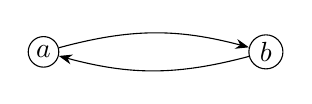
\begin{tikzpicture}[
  >={Stealth}, node distance=2.4cm,
  every node/.style={circle,draw,inner sep=1.5pt}
]
\node (a) {$a$};
\node (b) [right=of a] {$b$};
\draw[->] (a) to[bend left=15] (b);
\draw[->] (b) to[bend left=15] (a);
\end{tikzpicture}
\]
\textbf{False model (one-way arrow):}
\[
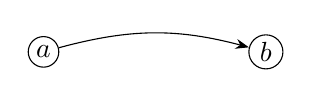
\begin{tikzpicture}[
  >={Stealth}, node distance=2.4cm,
  every node/.style={circle,draw,inner sep=1.5pt}
]
\node (a) {$a$};
\node (b) [right=of a] {$b$};
\draw[->] (a) to[bend left=15] (b);
\end{tikzpicture}
\]

\item $\forall x\forall y\exists z(Rxz\wedge Ryz)$

  \textbf{True model (common successor \(a\) for everyone):}
\[
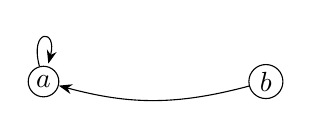
\begin{tikzpicture}[
  >={Stealth}, node distance=2.4cm,
  every node/.style={circle,draw,inner sep=1.5pt}
]
\node (a) {$a$};
\node (b) [right=of a] {$b$};
\draw[->] (a) edge[loop above] (a);
\draw[->] (b) to[bend left=15] (a);
\end{tikzpicture}
\]
(For any \(x,y\), choose \(z=a\).)

\textbf{False model (no common successor for \(a,b\)):}
\[
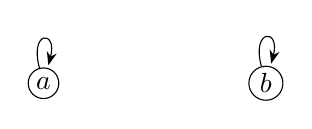
\begin{tikzpicture}[
  >={Stealth}, node distance=2.4cm,
  every node/.style={circle,draw,inner sep=1.5pt}
]
\node (a) {$a$};
\node (b) [right=of a] {$b$};
\draw[->] (a) edge[loop above] (a);
\draw[->] (b) edge[loop above] (b);
\end{tikzpicture}
\]
(For \(x=a,y=b\) there is no \(z\) with both \(a\to z\) and \(b\to z\).)

\item \(\exists x\forall y(Ryx\to Ryy)\)
  
\textbf{True model (choose \(x=a\) with no incoming arrows):}
\[
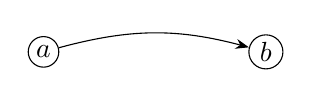
\begin{tikzpicture}[
  >={Stealth}, node distance=2.4cm,
  every node/.style={circle,draw,inner sep=1.5pt}
]
\node (a) {$a$};
\node (b) [right=of a] {$b$};
\draw[->] (a) to[bend left=15] (b);
\end{tikzpicture}
\]
(No \(y\) satisfies \(y\to a\), so \(Ryx\to Ryy\) holds vacuously for all \(y\).)

\textbf{False model (every \(x\) has an incoming arrow from a non-reflexive \(y\)):}
\[
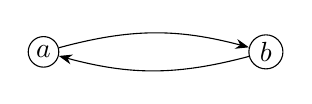
\begin{tikzpicture}[
  >={Stealth}, node distance=2.4cm,
  every node/.style={circle,draw,inner sep=1.5pt}
]
\node (a) {$a$};
\node (b) [right=of a] {$b$};
\draw[->] (a) to[bend left=15] (b);
\draw[->] (b) to[bend left=15] (a);
\end{tikzpicture}
\]
(No loops, so \(Ryy\) is always false; but each node has an incoming arrow.)

\item \(\forall x(\exists y\,Ryx \to \forall z\,Rzx)\)
  
\textbf{True model (empty relation):}
\[
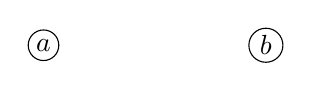
\begin{tikzpicture}[
  >={Stealth}, node distance=2.4cm,
  every node/.style={circle,draw,inner sep=1.5pt}
]
\node (a) {$a$};
\node (b) [right=of a] {$b$};
\end{tikzpicture}
\]
(Each antecedent \(\exists y\,Ryx\) is false, so the implication is true for all \(x\).)

\textbf{False model (some \(x\) has an incoming arrow but not everyone points to \(x\)):}
\[
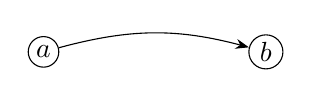
\begin{tikzpicture}[
  >={Stealth}, node distance=2.4cm,
  every node/.style={circle,draw,inner sep=1.5pt}
]
\node (a) {$a$};
\node (b) [right=of a] {$b$};
\draw[->] (a) to[bend left=15] (b);
\end{tikzpicture}
\]
(Take \(x=b\): \(\exists y\,Ryb\) holds (witness \(a\)), but \(\forall z\,Rzb\) fails since \(b\not\to b\).)

\item \(\exists x\exists y(Rxy \leftrightarrow \neg Ryy)\)
  
\textbf{True model (take \(x=a,y=b\)):}
\[
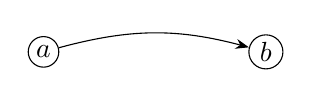
\begin{tikzpicture}[
  >={Stealth}, node distance=2.4cm,
  every node/.style={circle,draw,inner sep=1.5pt}
]
\node (a) {$a$};
\node (b) [right=of a] {$b$};
\draw[->] (a) to[bend left=15] (b);
\end{tikzpicture}
\]
(Here \(a\to b\) is true and \(b\to b\) is false, so \(\neg Rbb\) is true and the biconditional holds.)

\textbf{False model (universal relation on \(\{a,b\}\)):}
\[
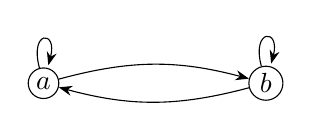
\begin{tikzpicture}[
  >={Stealth}, node distance=2.4cm,
  every node/.style={circle,draw,inner sep=1.5pt}
]
\node (a) {$a$};
\node (b) [right=of a] {$b$};
\draw[->] (a) edge[loop above] (a);
\draw[->] (b) edge[loop above] (b);
\draw[->] (a) to[bend left=15] (b);
\draw[->] (b) to[bend left=15] (a);
\end{tikzpicture}
\]
(For every \(y\), \(Ryy\) is true, hence \(\neg Ryy\) is false; but
\(Rxy\) is always true. So \(Rxy\leftrightarrow \neg Ryy\) is false
for all \(x,y\).)
\end{enumerate}

\exercise{8.8}
Yes, it is consistent.  Let the domain be $\mathbb{Z}$ and interpret $R$ as the strict order $<$.
Then $Rxx$ is never true, so $\neg Rxx$ holds for all $x$.
Given any $x\in\mathbb{Z}$, choose $y=x-1$.  Then $x<y$ is true, and for all $z$:
if $y<z$ then certainly $x<z$ (since $x<y<z$), so $(Ryz\to Rxz)$ holds.
Thus $\forall x\exists y\forall z(\neg Rxx\wedge Rxy\wedge(Ryz\to Rxz))$ is true in this model.

\exercise{8.9}
Two examples of sentences true in $(\mathbb{N},\le)$ but not consequences of the theory of
partial orders:

(1) ``There is a least element'':
\[
\exists x\,\forall y\,(x\le y).
\]
True in $(\mathbb{N},\le)$ (take $x=0$), but false in $(\mathbb{Z},\le)$, which is a partial order.

(2) ``The order is total'':
\[
\forall x\forall y\,\bigl(x\le y\;\vee\;y\le x\bigr).
\]
True in $(\mathbb{N},\le)$, but false in a poset with incomparable elements, e.g.\ a two-element
antichain where neither element is $\le$ the other.

\exercise{8.10}
Let $M$ be any interpretation.

(a) $[x,y:x=y]^M$ is the set of pairs $(a,b)\in M^2$ such that $a=b$, i.e.\ the diagonal:
\[
[x,y:x=y]^M=\{(a,a): a\in M\}\subseteq M^2.
\]

(b) $[x:x=x]^M$ is the set of $a\in M$ such that $a=a$, i.e.\ all of $M$:
\[
[x:x=x]^M = M.
\]

\exercise{8.11}
Attempting to mimic the proof for $\exists x\forall y(Fx\to Fy)$ breaks down in the case where
$F^M$ is neither empty nor all of $M$.

Indeed, take a countermodel: let the domain be $\{a,b\}$ and let $F^M=\{a\}$.
Then $Fa$ is true and $Fb$ is false, so $(Fa\to Fb)$ is false.  Hence
\[
\forall x\forall y(Fx\to Fy)
\]
fails in this interpretation.  Concretely, the universal quantifiers force us to check the
pair $x=a,y=b$, and at that point the implication is false.


\chaptersection{9}

\exercise{9.6}

Suppose that $\varphi$ is true in an even number $n$ of rows of its
truth table. Then $\neg \varphi$ is true in $4-n$ rows of its truth
table, and $4-n$ is also even.

Suppose that both $\varphi$ and $\psi$ are even. Let's say that row $r$ is an
\emph{agreement row} if $\varphi$ and $\psi$ have the same truth value on $r$. We
will show that there cannot be $1$ or $3$ agreement rows. Suppose that
there is a single row where both sentences have value $a$. Since $\varphi$ and
$\psi$ are even, $a$ must occur on another row in each of their truth
tables. If these rows are not the same, then there are two of them,
which leaves a single remaining row. In that row, both $\varphi$ and $\psi$ must
have value $1-a$, and so they agree there.

Suppose now that there are three rows where both sentences have the
same value, and let $r$ be the remaining row. Since three is odd, one
of the two truth values $a$ must occur most frequently on these
rows. If $a$ occurs twice and $1-a$ occurs once, then $1-a$ must be
the value of both $\varphi$ and $\psi$ on row $r$. If $a$ occurs three times, then
$a$ must be the value of both $\varphi$ and $\psi$ on row $r$. In either case, $\varphi$
and $\psi$ agree on row $r$.

\exercise{9.7}

No, the set $\{ \neg,\leftrightarrow \}$ is not truth-functionally
complete. There is a binary truth-function that has output a single
$1$ and three $0$. For example, take the sentence $P\wedge Q$. By
Exercise 9.6, every sentence in the set $\Gamma$ generated from $P,Q$
and $\{ \neg ,\leftrightarrow \}$ has an even number of $1$ in its
truth table. Therefore, there is no sentence in $\Gamma$ that is
provably equivalent to $P\wedge Q$.

\exercise{9.12}

Suppose that $\varphi$ is contingent, and let $P_0,\dots ,P_n$ be a
list of the atomic sentences that occur in $\varphi$. Since $\varphi$
is contingent, there is a valuation $v$ such that $v(\varphi )=0$. Let
$\bot$ be an arbitrary contradiction, and let $\top$ be an arbitrary
tautology. Define $F(P_i)=\top$ if $v(P_i)=1$, and $F(P_i)=\bot$ if
$v(P_i)=0$. We claim, then, that the substitution instance
$F(\varphi )$ is inconsistent. Let $w$ be an arbitrary valuation. For
any $P_i$, $w(F(P_i))=w(\top )=1$ if $v(P_i)=1$, and
$w(F(P_i))=w(\bot )=0$ if $v(P_i)=0$. So $w(F(\cdot ))$ and
$v(\cdot )$ agree on atomic sentences. But $w(F(\cdot ))$ and
$v(\cdot )$ are both truth-functional, so they agree on all
sentences. Therefore, $w(F(\varphi ))=v(\varphi )=0$. Since $w$ was
arbitrary, $F(\varphi )$ is an inconsistency.

\exercise{9.14}

\begin{enumerate}
\item As a warmup, we will show that all occurences of $\to$ can be
  eliminated from valid proofs, along with all uses of MP and
  CP. Define a function $f$ from sentences to sentences as the
  identity on atomic sentences, then extend by commuting with
  $\wedge ,\vee ,\neg$, and by setting
  $f(\varphi\to\psi )=\neg (f(\varphi )\wedge \neg f(\psi ))$. We now
  show that any proof of $\varphi _1,\dots ,\varphi _n\vdash \psi$ can
  be converted to a proof of
  $f(\varphi _1),\dots ,f(\varphi _n)\succ f(\psi )$.

  Here's a way to simulate CP. Suppose first that $\varphi$ is
  assumed, and that $\psi$ is derived with dependencies $\Delta$. We
  can then continue in this way:
  \noindent \[ \begin{array}{r|c|l|l}
1          & (1) & \varphi                      & \text{A} \\[2pt]
              \Delta     & (2) & \psi \\[6pt]
3          & (3) & \varphi \land \neg\psi       & \text{A} \\[2pt]
3          & (4) & \neg\psi                     & 3\ \land\text{E} \\[2pt]
\Delta,3   & (5) & \psi \land \neg\psi          & 2,4\ \land\text{I} \\[2pt]
\Delta',3  & (6) & \neg\varphi                  & 1,5\ \text{RA} \\[2pt]
3          & (7) & \varphi                      & 3\ \land\text{E} \\[2pt]
\Delta',3  & (8) & \varphi \land \neg\varphi    & 7,6\ \land\text{I} \\[2pt]
\Delta'    & (9) & \neg(\varphi \land \neg\psi) & 3,8\ \text{RA}
\end{array}
\]
Here $\Delta '=\Delta\setminus\{1\}$, so that line 9 reproduces the
effect of CP on lines 1 and 2.

Now we can simulate MP.
\noindent \[ \begin{array}{r|c|l|l}
               \Gamma     & (1) & \neg (\varphi\wedge \neg\psi) &  \\[2pt]
               \Delta     & (2) & \varphi \\[6pt]
               3          & (3) & \neg\psi                     & \text{A} \\[2pt]
               \Delta, 3  & (4) & \varphi\wedge\neg\psi        & 2,3\ \land\text{I} \\[2pt]
       \Gamma ,\Delta ,3  & (5) & (\varphi\wedge\neg\psi )\wedge\neg (\varphi\wedge\neg\psi)  & 4,1\ \land\text{I} \\[2pt]
       \Gamma ,\Delta     & (6) & \neg\neg\psi                  & 3,5\ \text{RA} \\[2pt]
        \Gamma ,\Delta    & (7) & \psi                          & 6\                                                                   \text{DN} \end{array}
\]
            
\item We need to show that any application of RA can be simulated by
  the other rules. Suppose that we have the following lines

\noindent \begin{tabular}{l >{\centering\arraybackslash}p{1.0cm} p{4cm} >{\raggedright\arraybackslash}p{3.5cm}}
\,1 & (1) & $P$ & A \\
$\Delta$ & (2) & $Q \wedge \neg Q$ \end{tabular}

\noindent We need to show that we can derive the line

\noindent \begin{tabular}{l >{\centering\arraybackslash}p{1.0cm} p{4cm} >{\raggedright\arraybackslash}p{3.5cm}}
            $\Delta '$ & ($c$) & $\neg P$ \end{tabular}

\noindent without using RA. We first derive $\Delta '\succ P\to\neg P$ as follows:
             
\noindent \begin{tabular}{l >{\centering\arraybackslash}p{1.0cm} p{4cm} >{\raggedright\arraybackslash}p{3.5cm}}
\,1 & (1) & $P$ & A \\
$\Delta$ & (2) & $Q \wedge \neg Q$ &  \\
$\Delta$ & (3) & $Q$ & 2 $\wedge$E \\
$\Delta '$ & (4) & $P \to Q$ & 1,3 CP \\
$\Delta$ & (5) & $\neg Q$ & 2 $\wedge$E \\
$\Delta$ & (6) & $\neg P$ & 4,5 MT \\
$\Delta '$ & (7) & $P \to \neg P$ & 1,6 CP \\
\end{tabular}

\noindent The proof that $\succ (P\to \neg P)\to \neg P$ is Exercise
3.1.10, plus one step of CP. Put those two together and $\Delta '\succ\neg P$ follows.

\item We show that the DN introduction rule can be reproduced from the
  other rules.

\noindent \begin{tabular}{r >{\centering\arraybackslash}p{1.0cm}
            p{4cm} >{\raggedright\arraybackslash}p{3.5cm}}
            1 & (1) & $P$ & A \\
            2 & (2) & $\neg P$ & A \\
            1,2 & (3) & $P\wedge\neg P$ & 1,2 $\wedge$I \\
            1 & (4) & $\neg\neg P$ & 2,3 RA \end{tabular}
             
\item We show that MT can be reproduced from the other rules.

\begin{tabular}{r >{\centering\arraybackslash}p{1.0cm} p{5cm} >{\raggedright\arraybackslash}p{3.5cm}}
1 & (1) & $P \to Q$ & A \\
2 & (2) & $\neg Q$ & A \\
3 & (3) & $P$ & A \\
1,3 & (4) & $Q$ & 1,3 MP \\
1,2,3 & (5) & $Q \wedge \neg Q$ & 4,2 $\wedge$I \\
1,2 & (6) & $\neg P$ & 3,5 RA \\
\end{tabular}

\item Redefine the truth-table for $\vee$ as follows:
  \[
\begin{array}{c c | c}
P & Q & P \vee Q \\
\hline
1 & 1 & 1 \\
1 & 0 & 1 \\
0 & 1 & 1 \\
0 & 0 & 1 \\
\end{array}
\]
In other words, $P\vee Q$ is constantly $1$, regardless of the
input. Since none of the inference rules besides $\vee$E uses a
disjunction as a premise, those rules are truth-preserving relative to
the new truth tables. We claim now that those rules cannot prove
$P\vee P\vdash P$. Consider the rows of the (new) truth-table in which
$P$ is $0$. In this case, $P\vee P$ is $1$, but $P$ is $0$. Hence
$P\vee P\vdash P$ is not truth-preserving relative to the new truth
tables, and it cannot be proven by those rules.

\item If we read this problem literally, then it admits trivial
  solutions. For example, we we permit ``nand'' statements to be
  inferred only from contradictions, and if permit only tautologies to
  be inferred from ``nand'' statement, then the resulting system of
  rules is sound. However, the spirit of this problem is to provide
  intro and elim rules for $\uparrow$ that capture the meaning of the
  connective.

%------------------ NAND INTRODUCTION ------------------
\subsubsection*{NAND-Introduction ($\uparrow$I)}

\noindent
If $\Delta$ together with $P$ and $Q$ imply $\bot$, then $\Delta$
implies $P\uparrow Q$.

\medskip

\begin{tabular}{c c l @{\hspace{3.5em}} l}
$a$   & ($a$)   & $P$ & A \\
$b$   & ($b$)   & $Q$ & A \\
$\Delta$ & ($c$) & $\bot$ &  \\[3pt]
$\Delta '$ & ($d$) & $P \uparrow Q$ & $a,b,c$ $\uparrow$I
\end{tabular}

\medskip \noindent where $\Delta '=\Delta -\{ a,b\}$.

%------------------ NAND ELIMINATION ------------------
\subsubsection*{NAND-Elimination ($\uparrow$E)}

\noindent From $P \uparrow Q$, together with $P$ and $Q$, infer $\bot$.

\medskip

\begin{tabular}{c c l @{\hspace{2.5em}} l}
$\Gamma$        & ($a$)   & $P \uparrow Q$ & \\ 
$\Delta$     & ($b$)   & $P$            & \\ 
$\Sigma$     & ($c$)   & $Q$            & \\[3pt]
$\Gamma,\Delta,\Sigma$ & ($d$) & $\bot$    & $a,b,c$ $\uparrow$E
\end{tabular}

%------------------ BOTTOM ELIMINATION ------------------
\subsubsection*{Falsum-Elimination ($\bot$E)}

For the $\uparrow$ rules to do enough, we need to add a
$\bot$-elimination rule.

\medskip

\begin{tabular}{r c l @{\hspace{2em}} l}
$\Gamma$ & ($a$)   & $\bot$ & \\[0.5em]
$\Gamma$ & ($b$) & $Q$    & $a$ $\bot$E
\end{tabular}


  

\end{enumerate}
  


\end{document}
%%% Local Variables:
%%% mode: latex
%%% TeX-master: t
%%% End:
